\documentclass[]{article}
\usepackage{lmodern}
\usepackage{amssymb,amsmath}
\usepackage{ifxetex,ifluatex}
\usepackage{fixltx2e} % provides \textsubscript
\ifnum 0\ifxetex 1\fi\ifluatex 1\fi=0 % if pdftex
  \usepackage[T1]{fontenc}
  \usepackage[utf8]{inputenc}
\else % if luatex or xelatex
  \ifxetex
    \usepackage{mathspec}
    \usepackage{xltxtra,xunicode}
  \else
    \usepackage{fontspec}
  \fi
  \defaultfontfeatures{Mapping=tex-text,Scale=MatchLowercase}
  \newcommand{\euro}{€}
\fi
% use upquote if available, for straight quotes in verbatim environments
\IfFileExists{upquote.sty}{\usepackage{upquote}}{}
% use microtype if available
\IfFileExists{microtype.sty}{%
\usepackage{microtype}
\UseMicrotypeSet[protrusion]{basicmath} % disable protrusion for tt fonts
}{}
\usepackage[margin=1in]{geometry}
\ifxetex
  \usepackage[setpagesize=false, % page size defined by xetex
              unicode=false, % unicode breaks when used with xetex
              xetex]{hyperref}
\else
  \usepackage[unicode=true]{hyperref}
\fi
\usepackage[usenames,dvipsnames]{color}
\hypersetup{breaklinks=true,
            bookmarks=true,
            pdfauthor={},
            pdftitle={Session 1 - Introduction.Rmd},
            colorlinks=true,
            citecolor=blue,
            urlcolor=blue,
            linkcolor=magenta,
            pdfborder={0 0 0}}
\urlstyle{same}  % don't use monospace font for urls
\usepackage{color}
\usepackage{fancyvrb}
\newcommand{\VerbBar}{|}
\newcommand{\VERB}{\Verb[commandchars=\\\{\}]}
\DefineVerbatimEnvironment{Highlighting}{Verbatim}{commandchars=\\\{\}}
% Add ',fontsize=\small' for more characters per line
\usepackage{framed}
\definecolor{shadecolor}{RGB}{248,248,248}
\newenvironment{Shaded}{\begin{snugshade}}{\end{snugshade}}
\newcommand{\AlertTok}[1]{\textcolor[rgb]{0.94,0.16,0.16}{#1}}
\newcommand{\AnnotationTok}[1]{\textcolor[rgb]{0.56,0.35,0.01}{\textbf{\textit{#1}}}}
\newcommand{\AttributeTok}[1]{\textcolor[rgb]{0.77,0.63,0.00}{#1}}
\newcommand{\BaseNTok}[1]{\textcolor[rgb]{0.00,0.00,0.81}{#1}}
\newcommand{\BuiltInTok}[1]{#1}
\newcommand{\CharTok}[1]{\textcolor[rgb]{0.31,0.60,0.02}{#1}}
\newcommand{\CommentTok}[1]{\textcolor[rgb]{0.56,0.35,0.01}{\textit{#1}}}
\newcommand{\CommentVarTok}[1]{\textcolor[rgb]{0.56,0.35,0.01}{\textbf{\textit{#1}}}}
\newcommand{\ConstantTok}[1]{\textcolor[rgb]{0.00,0.00,0.00}{#1}}
\newcommand{\ControlFlowTok}[1]{\textcolor[rgb]{0.13,0.29,0.53}{\textbf{#1}}}
\newcommand{\DataTypeTok}[1]{\textcolor[rgb]{0.13,0.29,0.53}{#1}}
\newcommand{\DecValTok}[1]{\textcolor[rgb]{0.00,0.00,0.81}{#1}}
\newcommand{\DocumentationTok}[1]{\textcolor[rgb]{0.56,0.35,0.01}{\textbf{\textit{#1}}}}
\newcommand{\ErrorTok}[1]{\textcolor[rgb]{0.64,0.00,0.00}{\textbf{#1}}}
\newcommand{\ExtensionTok}[1]{#1}
\newcommand{\FloatTok}[1]{\textcolor[rgb]{0.00,0.00,0.81}{#1}}
\newcommand{\FunctionTok}[1]{\textcolor[rgb]{0.00,0.00,0.00}{#1}}
\newcommand{\ImportTok}[1]{#1}
\newcommand{\InformationTok}[1]{\textcolor[rgb]{0.56,0.35,0.01}{\textbf{\textit{#1}}}}
\newcommand{\KeywordTok}[1]{\textcolor[rgb]{0.13,0.29,0.53}{\textbf{#1}}}
\newcommand{\NormalTok}[1]{#1}
\newcommand{\OperatorTok}[1]{\textcolor[rgb]{0.81,0.36,0.00}{\textbf{#1}}}
\newcommand{\OtherTok}[1]{\textcolor[rgb]{0.56,0.35,0.01}{#1}}
\newcommand{\PreprocessorTok}[1]{\textcolor[rgb]{0.56,0.35,0.01}{\textit{#1}}}
\newcommand{\RegionMarkerTok}[1]{#1}
\newcommand{\SpecialCharTok}[1]{\textcolor[rgb]{0.00,0.00,0.00}{#1}}
\newcommand{\SpecialStringTok}[1]{\textcolor[rgb]{0.31,0.60,0.02}{#1}}
\newcommand{\StringTok}[1]{\textcolor[rgb]{0.31,0.60,0.02}{#1}}
\newcommand{\VariableTok}[1]{\textcolor[rgb]{0.00,0.00,0.00}{#1}}
\newcommand{\VerbatimStringTok}[1]{\textcolor[rgb]{0.31,0.60,0.02}{#1}}
\newcommand{\WarningTok}[1]{\textcolor[rgb]{0.56,0.35,0.01}{\textbf{\textit{#1}}}}
\usepackage{graphicx,grffile}
\makeatletter
\def\maxwidth{\ifdim\Gin@nat@width>\linewidth\linewidth\else\Gin@nat@width\fi}
\def\maxheight{\ifdim\Gin@nat@height>\textheight\textheight\else\Gin@nat@height\fi}
\makeatother
% Scale images if necessary, so that they will not overflow the page
% margins by default, and it is still possible to overwrite the defaults
% using explicit options in \includegraphics[width, height, ...]{}
\setkeys{Gin}{width=\maxwidth,height=\maxheight,keepaspectratio}
\setlength{\parindent}{0pt}
\setlength{\parskip}{6pt plus 2pt minus 1pt}
\setlength{\emergencystretch}{3em}  % prevent overfull lines
\providecommand{\tightlist}{%
  \setlength{\itemsep}{0pt}\setlength{\parskip}{0pt}}
\setcounter{secnumdepth}{0}

\title{Session 1 - Introduction.Rmd}
\author{}
\date{\vspace{-2.5em}}

% Redefines (sub)paragraphs to behave more like sections
\ifx\paragraph\undefined\else
\let\oldparagraph\paragraph
\renewcommand{\paragraph}[1]{\oldparagraph{#1}\mbox{}}
\fi
\ifx\subparagraph\undefined\else
\let\oldsubparagraph\subparagraph
\renewcommand{\subparagraph}[1]{\oldsubparagraph{#1}\mbox{}}
\fi

\begin{document}
\maketitle

{
\hypersetup{linkcolor=black}
\setcounter{tocdepth}{2}
\tableofcontents
}
\hypertarget{the-purpose-of-this-course}{%
\section{The purpose of this course}\label{the-purpose-of-this-course}}

\begin{itemize}
\tightlist
\item
  An introduction to basic techniques in R
  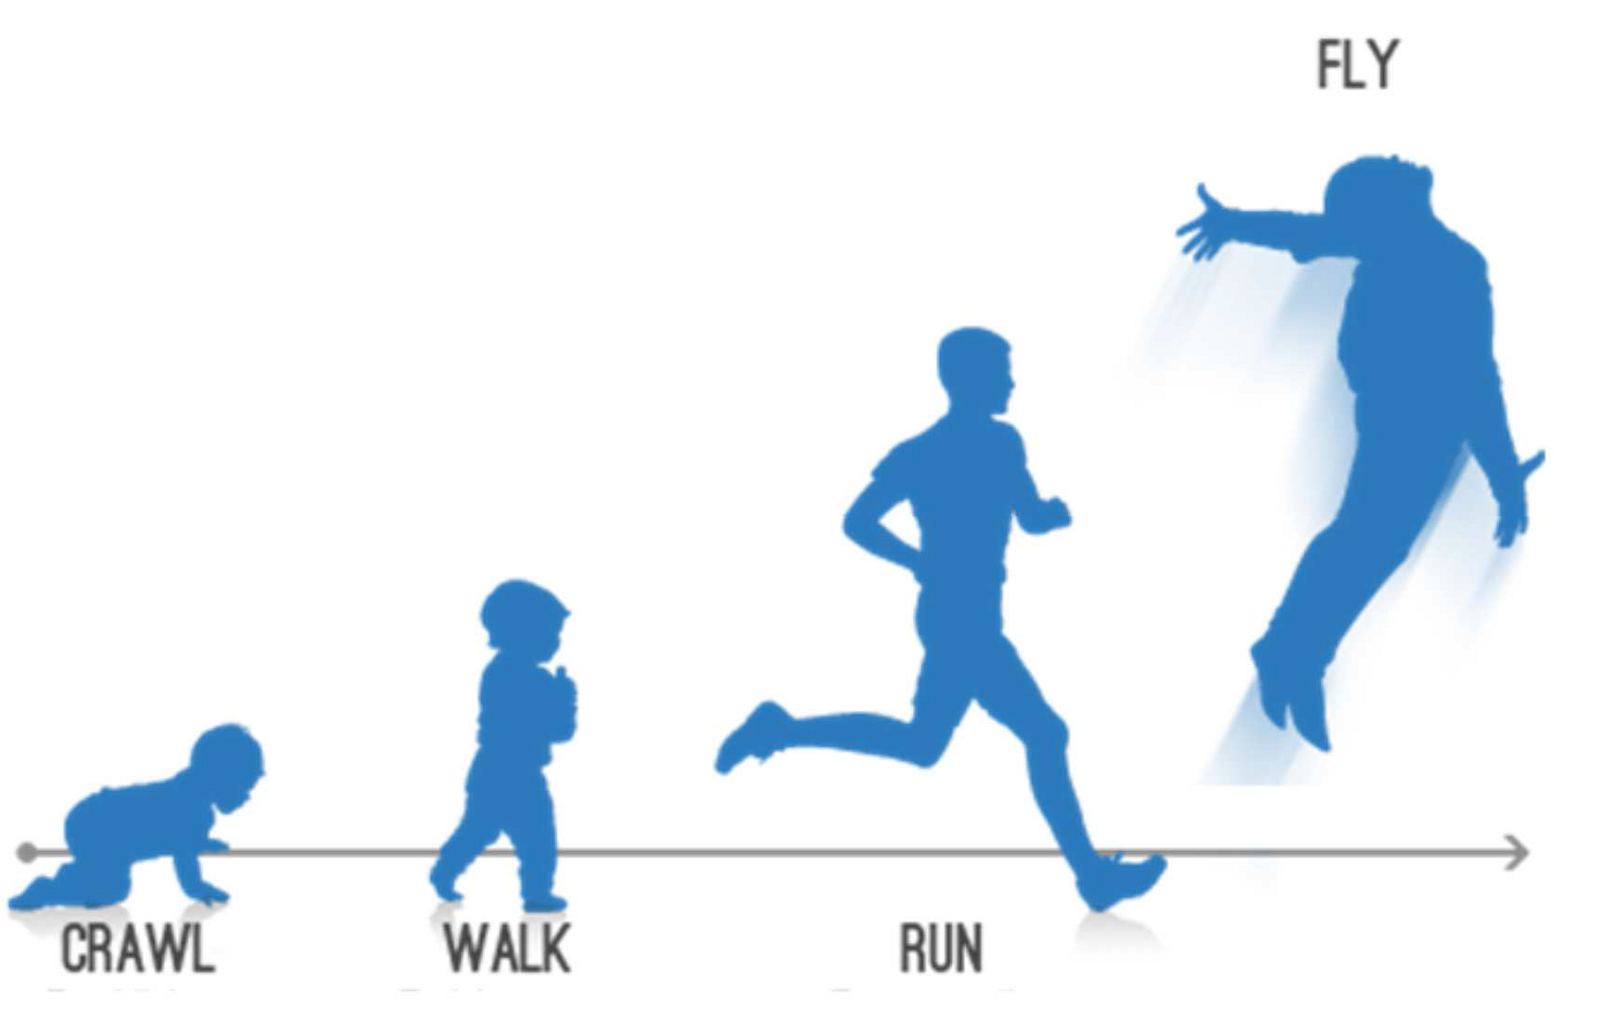
\includegraphics{crawl-walk-run-fly.png}
\item
  An interdisciplinary approach to R, e.g.~regression modelling for
  psychologists, and text analysis for digital humanities
\end{itemize}

\hypertarget{why-r}{%
\section{Why R?}\label{why-r}}

\begin{itemize}
\tightlist
\item
  \emph{Open Source}

  \begin{itemize}
  \tightlist
  \item
    means that analyses are (a) cutting edge and (b) accurate
  \end{itemize}
\item
  \emph{Strong emphasis on reproducible research}

  \begin{itemize}
  \tightlist
  \item
    data are (a) accurately reported (b) shareable
  \end{itemize}
\end{itemize}

\hypertarget{how-to-use-an-r-markdown-file}{%
\section{How to use an R Markdown
file}\label{how-to-use-an-r-markdown-file}}

This is an \href{http://rmarkdown.rstudio.com}{R Markdown} Notebook.
When you execute code within the notebook, the results appear beneath
the code.

Try executing this chunk by clicking the \emph{Run} button within the
chunk or by placing your cursor inside it and pressing
\emph{Ctrl+Shift+Enter}.

\begin{Shaded}
\begin{Highlighting}[]
\FunctionTok{plot}\NormalTok{(cars)}
\end{Highlighting}
\end{Shaded}

\includegraphics{Session_1_introduction_files/figure-latex/plot cars-1.pdf}

Add a new chunk by clicking the \emph{Insert} button on the toolbar or
by pressing \emph{Ctrl+Alt+I}.

When you save the notebook, an HTML file containing the code and output
will be saved alongside it (click the \emph{Preview} button or press
\emph{Ctrl+Shift+K} to preview the HTML file).

\begin{Shaded}
\begin{Highlighting}[]
\NormalTok{one }\OtherTok{\textless{}{-}} \DecValTok{1}
\NormalTok{one}
\end{Highlighting}
\end{Shaded}

\begin{verbatim}
## [1] 1
\end{verbatim}

\hypertarget{rstudio-breakdown}{%
\section{RStudio breakdown}\label{rstudio-breakdown}}

\hypertarget{panes}{%
\subsection{Panes}\label{panes}}

RStudio shows you four panes:

\begin{enumerate}
\def\labelenumi{\arabic{enumi}.}
\tightlist
\item
  The `Source' pane: the file where you write your code
\item
  The `Console' where actual code is run
\item
  The `Environment' pane, which shows you variables / datasets
\item
  The `Viewer' pane, which shows you plots and help files
\end{enumerate}

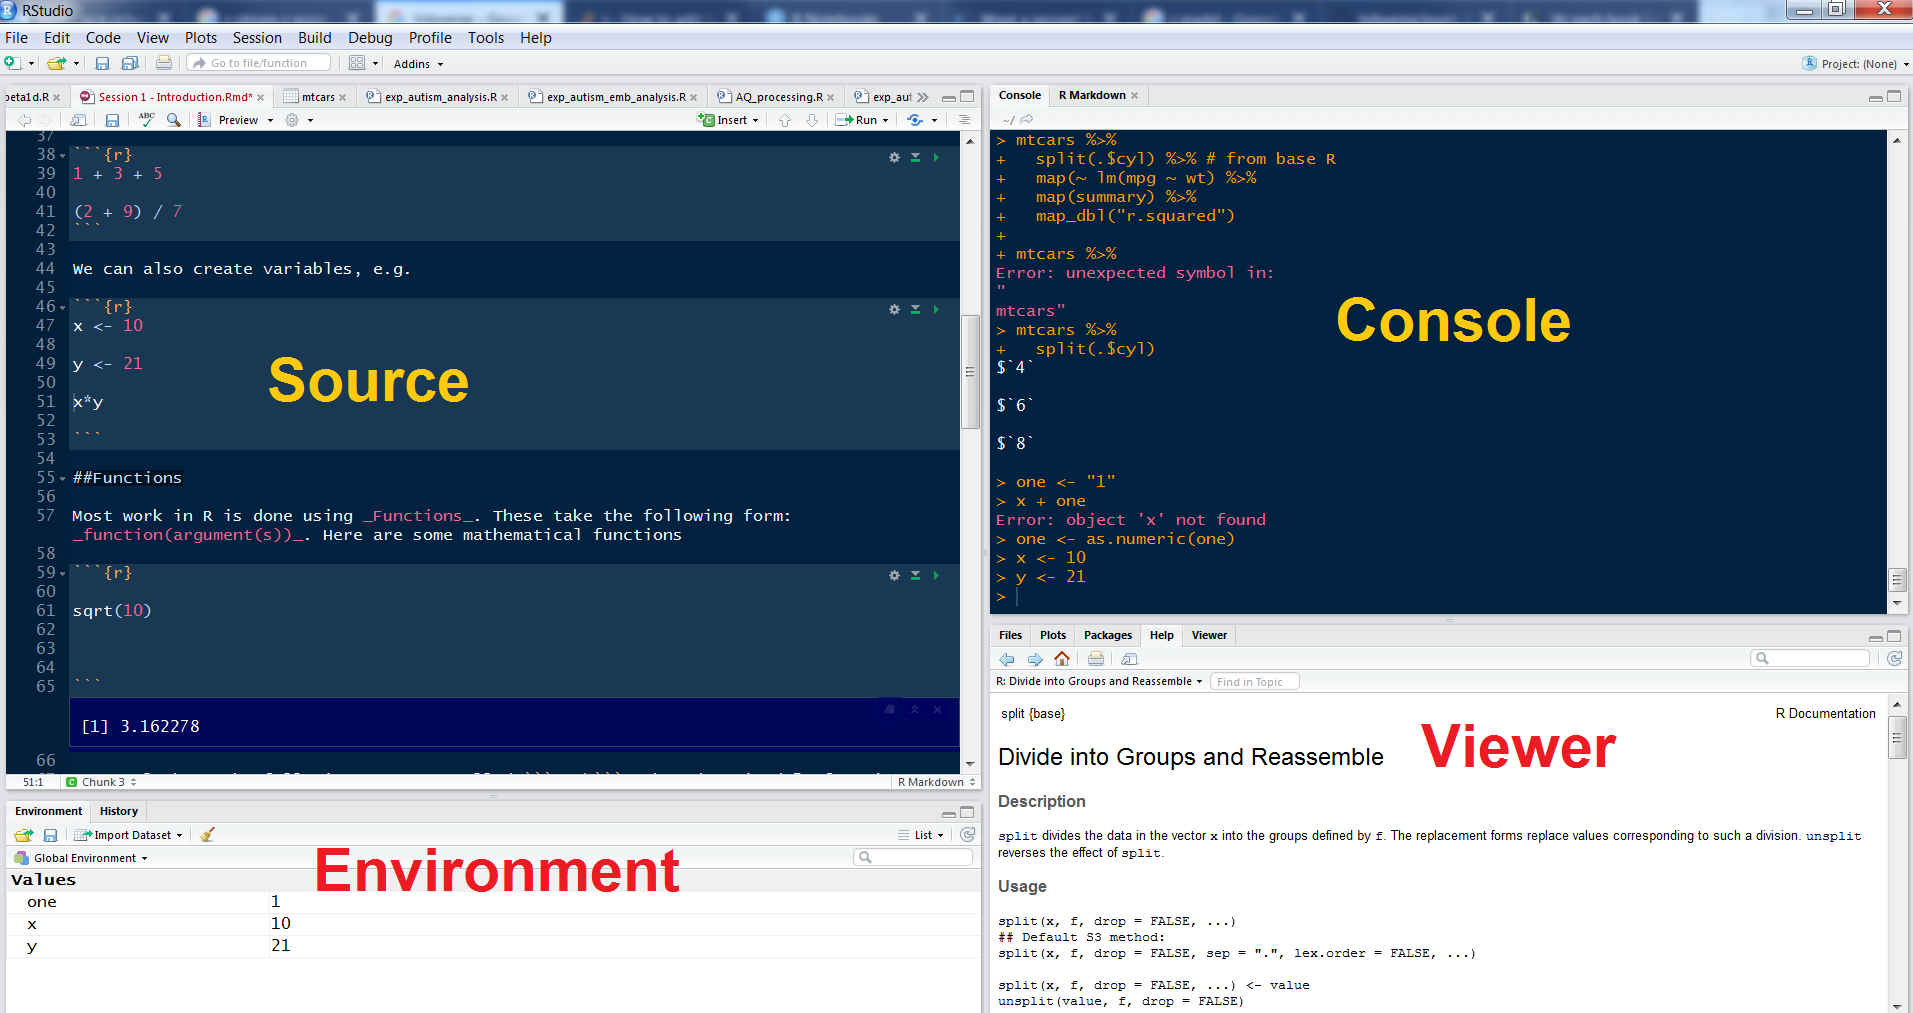
\includegraphics{console_etc.png}

You can arrange these in any order using Tools \textgreater{} Global
Options.

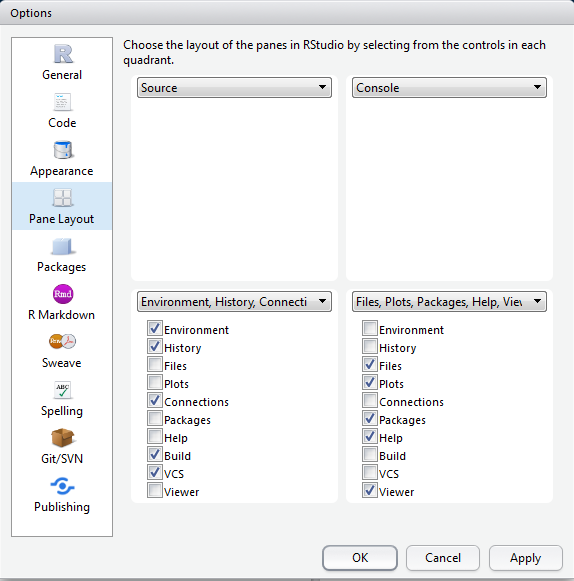
\includegraphics{panes.png}

\hypertarget{autocomplete}{%
\subsection{Autocomplete}\label{autocomplete}}

RStudio has fantastic autocomplete capabilites. To autocomplete just
press TAB. This is especially useful when loading files as using
autocomplete will help you to identify relevant ones. However it also
does lots of other things\ldots{}

\hypertarget{r-basics}{%
\section{R basics}\label{r-basics}}

\hypertarget{setting-the-working-directory}{%
\subsection{Setting the working
directory}\label{setting-the-working-directory}}

At the very beginning of an R session you MUST set a `working
directory'. This tells R where to look for and save files. An easy way
to do this is from RStudio. We're going to look at three ways to dos
this.

\hypertarget{the-easy-way}{%
\subsubsection{The easy way}\label{the-easy-way}}

Within
\texttt{RStudio\ go\ to\ Session\ \textgreater{}\textgreater{}\ Set\ Working\ Directory\ \textgreater{}\ Choose\ Directory...}

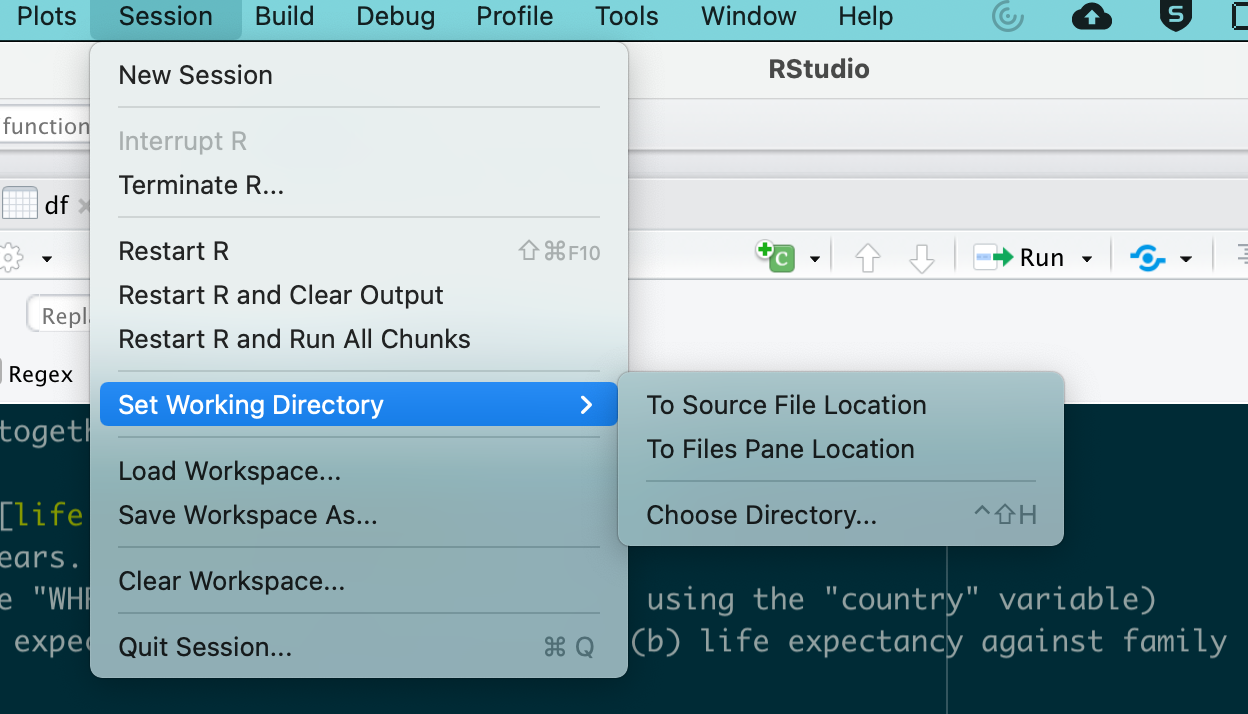
\includegraphics{setwd.png}

You also have an option to set the working directory to the most
recently-loaded \texttt{.R} or \texttt{.Rmd} file.

\hypertarget{the-difficult-way-1}{%
\subsubsection{The difficult way (1)}\label{the-difficult-way-1}}

To do this type

\texttt{setwd("path/to/directory")}

Unfortunately, if you are on a windows machine you will need to change
all backslashes \texttt{\textbackslash{}} to forward slashes \texttt{/}.
This is because R follows UNIX conventions which are native to Linux and
Mac computers.

If you are not sure what your working directory is type

\texttt{getwd()}

Getting the right path is a vital first step in R, and you really need
to know how to do this. Here are some instructional videos if you get
stuck\ldots{}

For Windows computers refer to
\href{https://www.youtube.com/watch?v=QzSV8wvA1Do}{this YouTube video}.
For Macs refer to
\href{https://www.youtube.com/watch?v=43W9TuPwqac}{this YouTube video}.
If you're on Linux then refer to
\href{https://www.youtube.com/watch?v=dQw4w9WgXcQ}{this YouTube video}

However this is a big problem with this approach. If you send your file
to someone else who is working on a different machine, it is most likely
that your path will be pointing to the wrong location

\hypertarget{the-difficult-way-2-but-by-far-the-best-way}{%
\subsubsection{The difficult way (2) (but by far the best
way!)}\label{the-difficult-way-2-but-by-far-the-best-way}}

By far the best way to set the working directory is create and ``R
Project'' in RStudio. When you do this, the RProject stores all files
and data objects which were opened in the last session, and also keeps
track of where the files are stored, so there is no need to set the
directory.

\hypertarget{using-r-as-a-calculator}{%
\subsection{Using R as a calculator}\label{using-r-as-a-calculator}}

We can use the console for general arithmetic

\begin{Shaded}
\begin{Highlighting}[]
\DecValTok{1} \SpecialCharTok{+} \DecValTok{3} \SpecialCharTok{+} \DecValTok{5}
\end{Highlighting}
\end{Shaded}

\begin{verbatim}
## [1] 9
\end{verbatim}

\begin{Shaded}
\begin{Highlighting}[]
\NormalTok{(}\DecValTok{2} \SpecialCharTok{+} \DecValTok{9}\NormalTok{) }\SpecialCharTok{/} \DecValTok{7}
\end{Highlighting}
\end{Shaded}

\begin{verbatim}
## [1] 1.571429
\end{verbatim}

\begin{Shaded}
\begin{Highlighting}[]
\DecValTok{1} \SpecialCharTok{+} \DecValTok{2}\SpecialCharTok{+} \DecValTok{3}
\end{Highlighting}
\end{Shaded}

\begin{verbatim}
## [1] 6
\end{verbatim}

We can also create variables, e.g.

\begin{Shaded}
\begin{Highlighting}[]
\NormalTok{x }\OtherTok{\textless{}{-}} \DecValTok{10} \CommentTok{\# This is a comment}
\NormalTok{x }\OtherTok{=} \DecValTok{10} \CommentTok{\# Does the same thing!!}
\NormalTok{y }\OtherTok{\textless{}{-}} \DecValTok{21}
\NormalTok{x}\SpecialCharTok{*}\NormalTok{y}
\end{Highlighting}
\end{Shaded}

\begin{verbatim}
## [1] 210
\end{verbatim}

\hypertarget{comments}{%
\subsection{Comments}\label{comments}}

If you'd like to comment on any code you write (i.e.~you do not wish R
to try to `run' this code) just add a hash (\texttt{\#}) or series of
hashes in front of it, e.g.

\begin{Shaded}
\begin{Highlighting}[]
\NormalTok{x }\OtherTok{\textless{}{-}} \DecValTok{100} \CommentTok{\# create a variable called x with the valuee 100}

\CommentTok{\# Now double it}

\NormalTok{x}\SpecialCharTok{*}\DecValTok{2}
\end{Highlighting}
\end{Shaded}

\begin{verbatim}
## [1] 200
\end{verbatim}

\hypertarget{functions}{%
\subsection{Functions}\label{functions}}

Most work in R is done using \emph{Functions}. These take the following
form: \emph{function(argument(s))}. Here are some functions

\begin{Shaded}
\begin{Highlighting}[]
\FunctionTok{sqrt}\NormalTok{(}\DecValTok{10}\NormalTok{)}
\end{Highlighting}
\end{Shaded}

\begin{verbatim}
## [1] 3.162278
\end{verbatim}

\begin{Shaded}
\begin{Highlighting}[]
\FunctionTok{seq}\NormalTok{(}\DecValTok{1}\NormalTok{, }\DecValTok{10}\NormalTok{, }\DecValTok{2}\NormalTok{)}
\end{Highlighting}
\end{Shaded}

\begin{verbatim}
## [1] 1 3 5 7 9
\end{verbatim}

\begin{Shaded}
\begin{Highlighting}[]
\FunctionTok{rep}\NormalTok{(}\DecValTok{5}\NormalTok{, }\DecValTok{10}\NormalTok{)}
\end{Highlighting}
\end{Shaded}

\begin{verbatim}
##  [1] 5 5 5 5 5 5 5 5 5 5
\end{verbatim}

\hypertarget{ex-1-2-working-with-functions}{%
\subsection{EX 1 \& 2: Working with
Functions}\label{ex-1-2-working-with-functions}}

EX1: What do the arguments of \texttt{seq} and \texttt{rep} do? To find
out more search for the relevant help file in the console by typing
\texttt{?seq} or by using Google.

EX2: Have a look at the following arguments called \texttt{gsub} and
\texttt{grepl}. What do they do? Clue: if you're stuck, search the help
file using \texttt{?}

\begin{Shaded}
\begin{Highlighting}[]
\FunctionTok{gsub}\NormalTok{(}\StringTok{"R{-}studio"}\NormalTok{, }\StringTok{"Rstudio"}\NormalTok{, }\StringTok{"R{-}studio is a great piece of software"}\NormalTok{)}
\end{Highlighting}
\end{Shaded}

\begin{verbatim}
## [1] "Rstudio is a great piece of software"
\end{verbatim}

\begin{Shaded}
\begin{Highlighting}[]
\FunctionTok{grepl}\NormalTok{(}\StringTok{"chocolate"}\NormalTok{, }\StringTok{"Mary likes chocolate cookies"}\NormalTok{)}
\end{Highlighting}
\end{Shaded}

\begin{verbatim}
## [1] TRUE
\end{verbatim}

\hypertarget{diy-functions}{%
\subsection{DIY functions}\label{diy-functions}}

It's possible to \textbf{create your own functions}. This makes R
extremely powerful and extendable. We're not going to cover making your
own functions in this course, but it's important to be aware of this
capability. There are plenty of good resources online for learning how
to do this, including
\href{https://www.statmethods.net/management/userfunctions.html}{this
one}

\hypertarget{getting-help}{%
\subsection{Getting help}\label{getting-help}}

As we have seen above, to find out about a particular function just type
\texttt{?} and the name of the function into the console,
e.g.~\texttt{?grepl}. This accesses the help files on your computer. If
you'd like to search more broadly type \texttt{??grepl} and your
computer will look online for relevant materials on CRAN (the main R
website)

Help files in R are quite densely written and not particularly aimed at
beginners. Fortunately there are loads of excellent resources on the
internet. Here are some really good sites:

\begin{enumerate}
\def\labelenumi{(\alph{enumi})}
\tightlist
\item
  \url{https://www.tidyverse.org/} - A brilliant set of of resources on
  all things related to the tidyverse, Hadley Wickham's brilliant suite
  of packages
\item
  \url{https://www.statmethods.net/index.html} - a quick way of looking
  up basic R techniques
\item
  \url{https://stats.idre.ucla.edu/r/modules/}
\item
  \url{https://rseek.org/} - a search engine for all things related to R
  (because the word `R' brings up a whole load of irrelevant stuff in
  Google)
\item
  \url{http://www.cookbook-r.com/} - this has lots of tips on how to do
  graphics.
\end{enumerate}

And there are plenty more! If you find a good one share it with your
colleagues via email, Twitter, or whatever social media you prefer!

\hypertarget{packages}{%
\section{Packages}\label{packages}}

\hypertarget{installation}{%
\subsection{Installation}\label{installation}}

To enhance the basic capabilities of R, we need to load
packages/libraries. Most of the time, we download these from `CRAN'
\texttt{Tools\ \textgreater{}\ Install\ packages} or
\texttt{install.packages()}. Once the package/library is installed
(i.e.~it is sitting somewhere on your computer), we then need to
\emph{load} it to the current R session using the \texttt{library()}
function.

Remember using a package/library is a two-stage process. We

\begin{enumerate}
\def\labelenumi{\arabic{enumi}.}
\tightlist
\item
  \emph{Install} the package/library onto your computer (from the
  internet)
\item
  \emph{Load} the package/library into your current session using the
  \texttt{library} command.
\end{enumerate}

One of the most useful packages is called `tidyverse'.

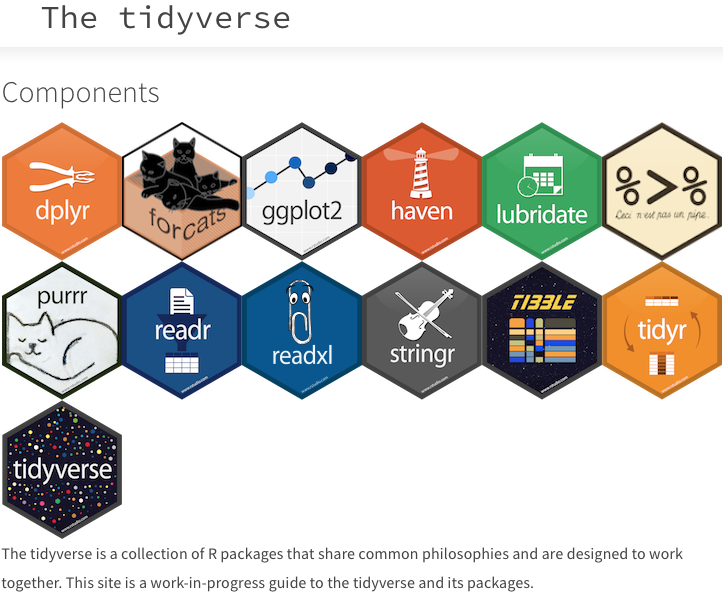
\includegraphics{tidyverse.png}

It contains a number of useful commands for plots, and data
manipulation.

Install the `tidyverse' package, and then load it with the following
function:

\begin{Shaded}
\begin{Highlighting}[]
\FunctionTok{library}\NormalTok{(tidyverse)}
\end{Highlighting}
\end{Shaded}

\begin{verbatim}
## -- Attaching packages --------------------------------------- tidyverse 1.3.1 --
\end{verbatim}

\begin{verbatim}
## v ggplot2 3.3.4     v purrr   0.3.4
## v tibble  3.1.7     v dplyr   1.0.9
## v tidyr   1.1.3     v stringr 1.4.0
## v readr   1.4.0     v forcats 0.5.1
\end{verbatim}

\begin{verbatim}
## Warning: package 'dplyr' was built under R version 4.1.2
\end{verbatim}

\begin{verbatim}
## -- Conflicts ------------------------------------------ tidyverse_conflicts() --
## x dplyr::filter() masks stats::filter()
## x dplyr::lag()    masks stats::lag()
\end{verbatim}

I find that a particularly easy way to load packages is via the
\texttt{p\_load} function from the \texttt{pacman} library. We are not
going to practise using it, but just to let you know that it exists!

\hypertarget{obtaining-help}{%
\subsection{Obtaining help}\label{obtaining-help}}

To find out more about a package type \texttt{?package\_name} in the
console. Alternatively you can look for the package documentation on
\href{https://cran.r-project.org/}{CRAN}.

\hypertarget{using-functions-from-packages}{%
\subsection{Using functions from
packages}\label{using-functions-from-packages}}

Most of the functions loaded in a package should work `out of the box'.
However occasionally you need to refer to the package first, and then
the function using the format
\texttt{package\_name::function\_from\_that\_package}. This is useful
for a variety of reasons:

\begin{enumerate}
\def\labelenumi{\arabic{enumi}.}
\tightlist
\item
  It allows you to use a function from a package without having to load
  that package (using the ``library'' commmand)
\item
  It helps in cases where you load two packages which contain two
  different functions which happen to have the same name.
\item
  Sometimes, even when a package is loaded, you need to precede a
  function by the package name. However, most of the time this is not
  necessary. (NB I am not sure why R sometimes requires the name of the
  package to be specified like this)
\end{enumerate}

\hypertarget{ex-3---using-packages}{%
\subsection{EX 3 - Using packages}\label{ex-3---using-packages}}

\begin{enumerate}
\def\labelenumi{\arabic{enumi}.}
\tightlist
\item
  Install and load the package \texttt{ggplot2}
\item
  Look up the function \texttt{geom\_point} from this package. What does
  it do?
\end{enumerate}

\hypertarget{objects-data-frames-and-indices}{%
\section{Objects, data frames and
indices}\label{objects-data-frames-and-indices}}

\hypertarget{objects}{%
\subsection{Objects}\label{objects}}

A variable is a type of `object' which R stores in memory. R is capable
of creating and storing a wide range of objects. To see what type of
object we have created, we use the function \texttt{class()}, e.g.

\begin{Shaded}
\begin{Highlighting}[]
\NormalTok{x }\OtherTok{\textless{}{-}} \DecValTok{1}

\FunctionTok{class}\NormalTok{(x)}
\end{Highlighting}
\end{Shaded}

\begin{verbatim}
## [1] "numeric"
\end{verbatim}

\begin{Shaded}
\begin{Highlighting}[]
\NormalTok{z }\OtherTok{\textless{}{-}} \StringTok{"hello"}

\FunctionTok{class}\NormalTok{(z)}
\end{Highlighting}
\end{Shaded}

\begin{verbatim}
## [1] "character"
\end{verbatim}

\emph{class} is one of the most useful functions in R as errors are
often due to misassignment of class, e.g.

\begin{Shaded}
\begin{Highlighting}[]
\NormalTok{x }\SpecialCharTok{+}\NormalTok{ z}
\end{Highlighting}
\end{Shaded}

\begin{verbatim}
## Error in x + z: non-numeric argument to binary operator
\end{verbatim}

Here we have tried to add a number to a string which is clearly
impossible. It's possible to change the class of an object using
commands such as \texttt{as.character}, \texttt{as.integer},
\texttt{as.numeric}, \texttt{as.factor}, e.g.

\begin{Shaded}
\begin{Highlighting}[]
\NormalTok{one }\OtherTok{\textless{}{-}} \StringTok{"1"}
\NormalTok{x }\SpecialCharTok{+}\NormalTok{ one}
\end{Highlighting}
\end{Shaded}

\begin{verbatim}
## Error in x + one: non-numeric argument to binary operator
\end{verbatim}

\begin{Shaded}
\begin{Highlighting}[]
\NormalTok{one }\OtherTok{\textless{}{-}} \FunctionTok{as.numeric}\NormalTok{(one)}
\NormalTok{x }\SpecialCharTok{+}\NormalTok{ one }
\end{Highlighting}
\end{Shaded}

\begin{verbatim}
## [1] 2
\end{verbatim}

Here is a visual summary of \emph{some} of the main data types / object
classes in R:

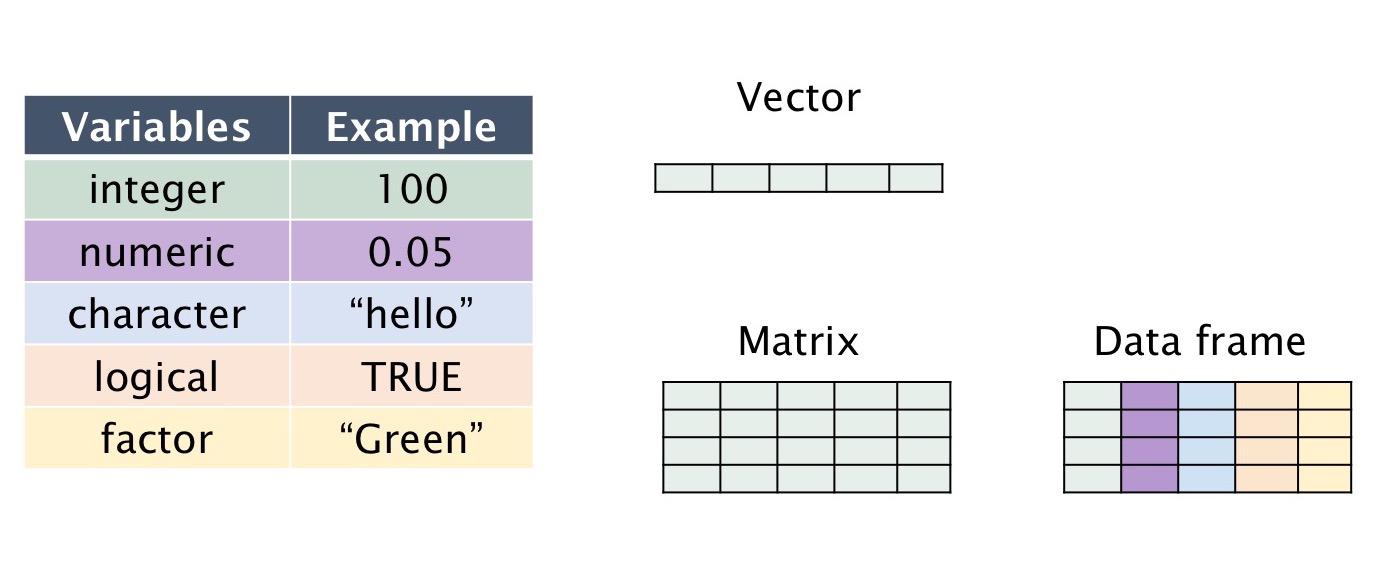
\includegraphics{data_types.jpeg}

Here are some definitions

\begin{enumerate}
\def\labelenumi{(\arabic{enumi})}
\tightlist
\item
  \emph{integer} = rounded number
\item
  \emph{numeric} = number with decimal points
\item
  \emph{character} = a string of characters
\item
  \emph{logical} = has a TRUE / FALSE value
\item
  \emph{factor} = a label which looks like a character variable, but
  which is mapped to a nominal variable, e.g.~``nationality''
\item
  \emph{vector} = a one-dimensional array where each position contains a
  different value from the same data type, e.g.~a series of numbers, or
  a series of words.
\item
  \emph{list} = a one-dimensional array where ach position contains a
  different value. Data types may \emph{vary}
\item
  \emph{matrix} = a two-dimensional array where all values are from the
  same data type
\item
  \emph{data frame} = a typical ``spreadsheet'' format. Columns are
  labelled. Columns may be of different types, e.g.~a column containing
  strings (characters), or a column containing numbers.
\end{enumerate}

In order to create a vector we need to use the \texttt{c} function. (c =
`combine'), e.g.

\begin{Shaded}
\begin{Highlighting}[]
\NormalTok{vector.of.numbers }\OtherTok{\textless{}{-}} \FunctionTok{c}\NormalTok{(}\DecValTok{1}\NormalTok{,}\DecValTok{4}\NormalTok{,}\DecValTok{54}\NormalTok{,}\DecValTok{22}\NormalTok{,}\DecValTok{43}\NormalTok{,}\DecValTok{9}\NormalTok{,}\DecValTok{0}\NormalTok{,}\DecValTok{0}\NormalTok{,}\DecValTok{21}\NormalTok{)}

\FunctionTok{mean}\NormalTok{(vector.of.numbers)}
\end{Highlighting}
\end{Shaded}

\begin{verbatim}
## [1] 17.11111
\end{verbatim}

\begin{Shaded}
\begin{Highlighting}[]
\FunctionTok{sd}\NormalTok{(vector.of.numbers)}
\end{Highlighting}
\end{Shaded}

\begin{verbatim}
## [1] 19.85223
\end{verbatim}

\begin{Shaded}
\begin{Highlighting}[]
\NormalTok{a.character.vector }\OtherTok{\textless{}{-}} \FunctionTok{c}\NormalTok{(}\StringTok{"Mary"}\NormalTok{, }\StringTok{"Jane"}\NormalTok{, }\StringTok{"Ali"}\NormalTok{, }\StringTok{"Chen"}\NormalTok{)}

\NormalTok{a.list }\OtherTok{\textless{}{-}} \FunctionTok{as.list}\NormalTok{(}\FunctionTok{c}\NormalTok{(}\DecValTok{1}\NormalTok{, }\DecValTok{2}\NormalTok{, }\StringTok{"Mary"}\NormalTok{, }\StringTok{"Jane"}\NormalTok{))}
\end{Highlighting}
\end{Shaded}

\hypertarget{creating-a-data-frame-from-scratch}{%
\subsection{Creating a data frame from
scratch}\label{creating-a-data-frame-from-scratch}}

A data frame is a two-dimensional object containing variables and row
numbers. It's basically a spreadsheet.

The following code creates a data frame programmatically. It creates two
variables, and combines them together to make a data frame. Note that to
do this we need to use the functions \texttt{as.data.frame} and
\texttt{cbind}.

\begin{Shaded}
\begin{Highlighting}[]
\NormalTok{list.of.movies }\OtherTok{\textless{}{-}} \FunctionTok{c}\NormalTok{(}\StringTok{"Independence Day"}\NormalTok{, }\StringTok{"Pretty Woman"}\NormalTok{, }\StringTok{"The Godfather Part}
\StringTok{Two"}\NormalTok{, }\StringTok{"Planet of the Apes (original)"}\NormalTok{)}

\NormalTok{rotten.tomatoes.variable }\OtherTok{\textless{}{-}} \FunctionTok{c}\NormalTok{(}\DecValTok{62}\NormalTok{, }\DecValTok{61}\NormalTok{, }\DecValTok{97}\NormalTok{, }\DecValTok{89}\NormalTok{)}

\NormalTok{df }\OtherTok{\textless{}{-}} \FunctionTok{as.data.frame}\NormalTok{(}\FunctionTok{cbind}\NormalTok{(list.of.movies, rotten.tomatoes.variable)) }\CommentTok{\# \textquotesingle{}cbind\textquotesingle{} binds columns together}
\end{Highlighting}
\end{Shaded}

\hypertarget{viewing-the-contents-of-a-data-frame}{%
\subsection{Viewing the contents of a data
frame}\label{viewing-the-contents-of-a-data-frame}}

To glimpse the top few rows type \texttt{head(name\_of\_data\_frame)} in
the console, e.g.

\begin{Shaded}
\begin{Highlighting}[]
\FunctionTok{head}\NormalTok{(df)}
\end{Highlighting}
\end{Shaded}

\begin{verbatim}
##                  list.of.movies rotten.tomatoes.variable
## 1              Independence Day                       62
## 2                  Pretty Woman                       61
## 3       The Godfather Part\nTwo                       97
## 4 Planet of the Apes (original)                       89
\end{verbatim}

To view the data frame in the `source' window, type
\texttt{View(name\_of\_data\_frame)} in the console, .e.g.

\begin{Shaded}
\begin{Highlighting}[]
\FunctionTok{View}\NormalTok{(df) }\CommentTok{\#NB first letter is a capital letter.}
\end{Highlighting}
\end{Shaded}

\hypertarget{referring-to-variables}{%
\subsection{Referring to variables}\label{referring-to-variables}}

To refer to variables, use the following syntax
\texttt{data\_frame\_name\$variable\_name}, e.g.

\begin{Shaded}
\begin{Highlighting}[]
\NormalTok{df}\SpecialCharTok{$}\NormalTok{list.of.movies}
\end{Highlighting}
\end{Shaded}

\begin{verbatim}
## [1] "Independence Day"              "Pretty Woman"                 
## [3] "The Godfather Part\nTwo"       "Planet of the Apes (original)"
\end{verbatim}

When naming variables we can use dots and underscores,
e.g.~\texttt{df\$list.of.movies} and \texttt{df\$list\_of\_movies}. We
can use numbers as long as they don't come at the beginning,
e.g.~\texttt{df\$list\_of\_movies.v3}.

If you use this convention, then the names for variables can get very
long. However, it's generally useful, as in R you often have multiple
data frames loaded into memory. By specifiying both the name of the data
frame and the variable, this avoids confusion.

Try to be consistent with your naming conventions. I tend to use
underscores to name variables, e.g.~\texttt{data.frame.x\$variable\_y}.
This is also what Hadley Wickham recommends (Have a look at the
\href{https://style.tidyverse.org/}{Tidyverse Style Guide})

If you'd like to see all the variable names in a data frame type
\texttt{names(data\_frame)}, e.g.~

\begin{Shaded}
\begin{Highlighting}[]
\FunctionTok{names}\NormalTok{(df)}
\end{Highlighting}
\end{Shaded}

\begin{verbatim}
## [1] "list.of.movies"           "rotten.tomatoes.variable"
\end{verbatim}

\hypertarget{indices}{%
\subsection{Indices}\label{indices}}

Whenever you wish to access the contents of an object with multiple
values (e.g.~a data frame) you use indexes. These are placed inside
square brackets, e.g.~\texttt{{[}1{]}}. Have a look at the following
example:

\begin{Shaded}
\begin{Highlighting}[]
\NormalTok{df[}\DecValTok{1}\NormalTok{,}\DecValTok{2}\NormalTok{]}
\end{Highlighting}
\end{Shaded}

\begin{verbatim}
## [1] "62"
\end{verbatim}

\begin{Shaded}
\begin{Highlighting}[]
\NormalTok{df[}\DecValTok{1}\NormalTok{,] }\CommentTok{\# here the second number is blank}
\end{Highlighting}
\end{Shaded}

\begin{verbatim}
##     list.of.movies rotten.tomatoes.variable
## 1 Independence Day                       62
\end{verbatim}

\begin{Shaded}
\begin{Highlighting}[]
\NormalTok{df[,}\DecValTok{2}\NormalTok{] }\CommentTok{\# here the first number is blank}
\end{Highlighting}
\end{Shaded}

\begin{verbatim}
## [1] "62" "61" "97" "89"
\end{verbatim}

Below is a diagram demonstrating how indices work.

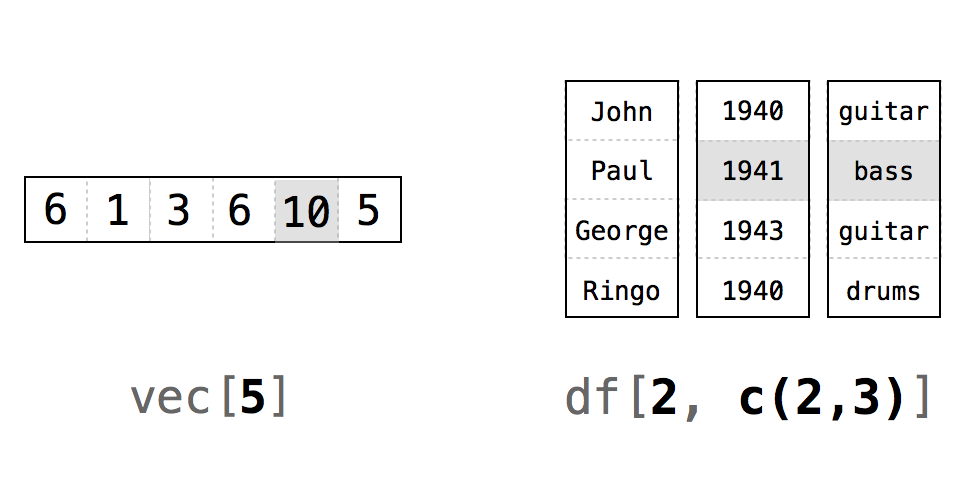
\includegraphics{indices.png}

\hypertarget{ex-3---understanding-indices}{%
\subsection{EX 3 - understanding
indices}\label{ex-3---understanding-indices}}

What does each number refer to? What happens when we leave a blank cell?

\hypertarget{reading-data-frames-from-files-using-menus}{%
\subsection{Reading data frames from files using
menus}\label{reading-data-frames-from-files-using-menus}}

We can use the menu in Rstudio:
\texttt{File\ \textgreater{}\ Import\ dataset}. You can do this to
import Excel, SPSS, SAS and STATA files.

\hypertarget{reading-data-frames-from-files-using-code}{%
\subsection{Reading data frames from files using
code}\label{reading-data-frames-from-files-using-code}}

However, rather than use the menu, it's much better to use actual code,
as this will automate the process. Let's import a dataset on World
Happiness Report (2017), by country. The files are \url{WHR_2019.xlsx},
and \url{WHR_2019.csv}. Alternatively you can actually download the data
set straight from the URL (below)

\begin{Shaded}
\begin{Highlighting}[]
\FunctionTok{library}\NormalTok{(tidyverse)}

\NormalTok{df }\OtherTok{\textless{}{-}}\NormalTok{ readxl}\SpecialCharTok{::}\FunctionTok{read\_excel}\NormalTok{(}\StringTok{"WHR\_2019.xlsx"}\NormalTok{) }\CommentTok{\# Read an excel file}

\NormalTok{df }\OtherTok{\textless{}{-}} \FunctionTok{read\_csv}\NormalTok{(}\StringTok{"WHR\_2019.csv"}\NormalTok{) }\CommentTok{\# Read from a .csv file}

\CommentTok{\# Or to download straight from the URL!!}

\CommentTok{\# df \textless{}{-} read\_csv("https://verbingnouns.github.io/AdventuresInR/docs/WHR\_2017.csv")}

\CommentTok{\# This code adds a region variable for each country. Don\textquotesingle{}t worry about how the code works. We will come back go it later!!}

\NormalTok{df.regions }\OtherTok{\textless{}{-}}\NormalTok{ readxl}\SpecialCharTok{::}\FunctionTok{read\_excel}\NormalTok{(}\StringTok{"countries\_and\_regions.xlsx"}\NormalTok{)}

\NormalTok{df }\SpecialCharTok{\%\textgreater{}\%} \FunctionTok{merge}\NormalTok{(df.regions) }\OtherTok{{-}\textgreater{}}\NormalTok{ df}
\end{Highlighting}
\end{Shaded}

Possibly the best data format to work in is the .csv data format
(Comma-Separated Value). This is good because it is readable in Excel,
small, simple, and not easily-corrupted.

To read .csv files we use the \texttt{read.csv()} function from base R,
or \texttt{read\_csv()} from the tidyverse (I would go with the latter
as it also shows you a list of the variable types)

\hypertarget{subsetting-a-data-set-using-a-base-r-and-d-dplyr}{%
\section{Subsetting a data set using (a) base R and (d)
dplyr}\label{subsetting-a-data-set-using-a-base-r-and-d-dplyr}}

\hypertarget{subsetting-with-base-r}{%
\subsection{Subsetting with base R}\label{subsetting-with-base-r}}

We're going to \emph{subset} the WHR dataset (i.e.~choose only those
cases/observations which fulfil a specific criterion). To do this we're
going to use the \texttt{which()} function. When you apply
\texttt{which} to a variable in a dataset, it will produce indices
(indexes) of the rows which fulfil a certain criterio,
e.g.~\texttt{which(df\$var\_name\ ==\ 2)} will give you the indices of
all rows where the value of the variable is 2.

\hypertarget{ex4-subsetting-the-hard-way}{%
\subsection{EX4: Subsetting the hard
way!}\label{ex4-subsetting-the-hard-way}}

Armed with this knowledge, your task is to subset the data frame so that
it only contains information from African countries.

If you're stuck have a look at the answer below.

\begin{Shaded}
\begin{Highlighting}[]
\NormalTok{df.Africa }\OtherTok{\textless{}{-}}\NormalTok{ df[}\FunctionTok{which}\NormalTok{(df}\SpecialCharTok{$}\NormalTok{region }\SpecialCharTok{==} \StringTok{"Africa"}\NormalTok{), ]}
\end{Highlighting}
\end{Shaded}

\hypertarget{piping}{%
\subsection{Piping}\label{piping}}

Okay, the above code is pretty horrible to look at, so we're going to
explore an alternative using the package \texttt{dplyr} which is from
the \texttt{tidyverse}. But before we can use \texttt{dplyr} we have to
learn how to `pipe'.


\includegraphics{MagrittePipe.jpg}

Pipes are written in R as \texttt{\%\textgreater{}\%} (note you must use
a percentage sign before and after the pipe). To demonstrate what pipes
do, I have a look at the following pseudocode.

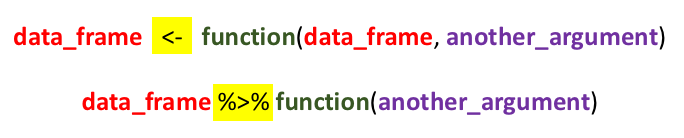
\includegraphics{piping.png}

All pipes do is enable us to `pass' a data frame (or another object) to
a new function without having to keep on specifying the data frame. In
addition, we can \emph{chain} pipes together indefinitely.

Here's how we would subset the data frame using piping:

\begin{Shaded}
\begin{Highlighting}[]
\NormalTok{df.Africa }\OtherTok{\textless{}{-}} \FunctionTok{filter}\NormalTok{(df, region }\SpecialCharTok{==} \StringTok{"Africa"}\NormalTok{) }\CommentTok{\# This is the version without piping}

\NormalTok{df }\SpecialCharTok{\%\textgreater{}\%} \FunctionTok{filter}\NormalTok{(region }\SpecialCharTok{==} \StringTok{"Africa"}\NormalTok{) }\OtherTok{{-}\textgreater{}}\NormalTok{ df.Africa }\CommentTok{\# This is the version with piping. It looks longer, but we can chain multiple functions together!}
\end{Highlighting}
\end{Shaded}

Note that to create a new data frame, we need a solid arrow at the end.
If we don't include that solid arrow, the results are shown in the
console, but no new data frame is created. This is an incredibly useful
feature of pipes. You can \texttt{try\ before\ you\ buy}!

And here is an example where we \emph{chain} a series of pipes together:

\begin{Shaded}
\begin{Highlighting}[]
\NormalTok{df.new }\OtherTok{\textless{}{-}} \FunctionTok{read\_csv}\NormalTok{(}\StringTok{"WHR\_2019.csv"}\NormalTok{)}
\end{Highlighting}
\end{Shaded}

\begin{verbatim}
## 
## -- Column specification --------------------------------------------------------
## cols(
##   rank = col_double(),
##   country = col_character(),
##   happiness_score = col_double(),
##   gdp_per_capita = col_double(),
##   social_support = col_double(),
##   healthy_life_expectancy = col_double(),
##   freedom = col_double(),
##   generosity = col_double(),
##   perceptions_of_corruption = col_double()
## )
\end{verbatim}

\begin{Shaded}
\begin{Highlighting}[]
\NormalTok{df.new }\SpecialCharTok{\%\textgreater{}\%} 
  \FunctionTok{merge}\NormalTok{(df.regions) }\SpecialCharTok{\%\textgreater{}\%} 
  \FunctionTok{group\_by}\NormalTok{(region) }\SpecialCharTok{\%\textgreater{}\%}
  \FunctionTok{summarise}\NormalTok{(}\AttributeTok{mean.happiness =} \FunctionTok{mean}\NormalTok{(happiness\_score)) }\OtherTok{{-}\textgreater{}}
\NormalTok{  df.mean.happiness.by.region}
\end{Highlighting}
\end{Shaded}

NB When piping the code becomes more readable when the line ends with
the pipe.

There are a couple of important points to note.

\begin{enumerate}
\def\labelenumi{(\arabic{enumi})}
\tightlist
\item
  We can refer to variables without specifying the data frame
\item
  If we wish to store the results we must output them using and arrow
  \texttt{-\textgreater{}}. If we don't store the results they will
  merely be displayed in the console.
\end{enumerate}

Piping is a key technique in R and once you've learnt it you will write
much more powerful and readable code.

As well as using pipes to create data frame, you can also insert pipes
into both analyses and figures! Here are some examples

\begin{Shaded}
\begin{Highlighting}[]
\CommentTok{\# An ANOVA without a pipe. NB we are using the base function "aov". If you would like to conduct SPSS{-}style ANOVAs, the best package is called "afex".}



\NormalTok{mod }\OtherTok{\textless{}{-}} \FunctionTok{aov}\NormalTok{(rank }\SpecialCharTok{\textasciitilde{}}\NormalTok{ region, }\AttributeTok{data =}\NormalTok{ df)}

\NormalTok{pacman}\SpecialCharTok{::}\FunctionTok{p\_load}\NormalTok{(broom) }\CommentTok{\# To load the "tidy" function.}

\FunctionTok{tidy}\NormalTok{(mod)}
\end{Highlighting}
\end{Shaded}

\begin{verbatim}
## # A tibble: 2 x 6
##   term         df   sumsq meansq statistic   p.value
##   <chr>     <dbl>   <dbl>  <dbl>     <dbl>     <dbl>
## 1 region        9 173153. 19239.      20.5  1.73e-21
## 2 Residuals   137 128837.   940.      NA   NA
\end{verbatim}

\begin{Shaded}
\begin{Highlighting}[]
\CommentTok{\# Here we use a pipe inside the analysis}
\NormalTok{mod }\OtherTok{\textless{}{-}} \FunctionTok{aov}\NormalTok{(rank }\SpecialCharTok{\textasciitilde{}}\NormalTok{ region, }\CommentTok{\# NB note we can break the line after a comma}
           \AttributeTok{data =}\NormalTok{ df }\SpecialCharTok{\%\textgreater{}\%} \FunctionTok{filter}\NormalTok{(region }\SpecialCharTok{==} \StringTok{"Africa"} \SpecialCharTok{|}\NormalTok{ region }\SpecialCharTok{==} \StringTok{"South America"}\NormalTok{))}

\FunctionTok{tidy}\NormalTok{(mod)}
\end{Highlighting}
\end{Shaded}

\begin{verbatim}
## # A tibble: 2 x 6
##   term         df  sumsq meansq statistic   p.value
##   <chr>     <dbl>  <dbl>  <dbl>     <dbl>     <dbl>
## 1 region        1 52918. 52918.      119.  2.25e-14
## 2 Residuals    46 20388    443.       NA  NA
\end{verbatim}

\begin{Shaded}
\begin{Highlighting}[]
\NormalTok{g }\OtherTok{\textless{}{-}} \FunctionTok{ggplot}\NormalTok{(}\FunctionTok{aes}\NormalTok{(}\AttributeTok{x =}\NormalTok{ gdp\_per\_capita, }\AttributeTok{y =}\NormalTok{ happiness\_score, }\AttributeTok{colour =}\NormalTok{ region), }\CommentTok{\# NB note we can break the line after a comma}
            \AttributeTok{data =}\NormalTok{ df }\SpecialCharTok{\%\textgreater{}\%} \FunctionTok{filter}\NormalTok{(region }\SpecialCharTok{==} \StringTok{"Africa"} \SpecialCharTok{|}\NormalTok{ region }\SpecialCharTok{==} \StringTok{"South America"}\NormalTok{))}
\NormalTok{g }\OtherTok{\textless{}{-}}\NormalTok{ g }\SpecialCharTok{+} \FunctionTok{geom\_point}\NormalTok{()}
\NormalTok{g }\OtherTok{\textless{}{-}}\NormalTok{ g }\SpecialCharTok{+} \FunctionTok{geom\_smooth}\NormalTok{(}\AttributeTok{method =} \StringTok{"lm"}\NormalTok{)}
\NormalTok{g}
\end{Highlighting}
\end{Shaded}

\begin{verbatim}
## `geom_smooth()` using formula 'y ~ x'
\end{verbatim}

\includegraphics{Session_1_introduction_files/figure-latex/using pipes inside statistical models and plots-1.pdf}

Note how I have broken some of the lines after a comma. This makes the
code more readable. Generally we can break a line when it ends in some
kind of symbol, e.g.~a pipe, an arrow, or a comma.

\hypertarget{loops-and-if-then-statements}{%
\section{Loops and if-then
statements}\label{loops-and-if-then-statements}}

Loops and if-then statements are useful programming tools which have the
same structure: \texttt{FUNCTION\ (STATEMENT)\ \{.....\}}.

\hypertarget{loops}{%
\subsection{Loops}\label{loops}}

\includegraphics{https://media.giphy.com/media/MDXomrcGshGso/giphy.gif}

\begin{Shaded}
\begin{Highlighting}[]
\ControlFlowTok{for}\NormalTok{(i }\ControlFlowTok{in} \DecValTok{1}\SpecialCharTok{:}\DecValTok{10}\NormalTok{)\{}
  \FunctionTok{print}\NormalTok{(}\FunctionTok{as.character}\NormalTok{(i))}
\NormalTok{\}}
\end{Highlighting}
\end{Shaded}

\begin{verbatim}
## [1] "1"
## [1] "2"
## [1] "3"
## [1] "4"
## [1] "5"
## [1] "6"
## [1] "7"
## [1] "8"
## [1] "9"
## [1] "10"
\end{verbatim}

To demonstrate a loop we're going to look at the WHR data set. We're
going to ask the question 'for different regions of the world, what is
the relationship between GDP per capita nd happiness?

Here's how we would do it

\begin{Shaded}
\begin{Highlighting}[]
\CommentTok{\# This code drops regions where number of observations are less than 3 (we can\textquotesingle{}t do correlations if there are less than 3 observations)}

\NormalTok{df }\SpecialCharTok{\%\textgreater{}\%}
  \FunctionTok{group\_by}\NormalTok{(region) }\SpecialCharTok{\%\textgreater{}\%}
  \FunctionTok{summarise}\NormalTok{(}\AttributeTok{num =} \FunctionTok{n}\NormalTok{()) }\SpecialCharTok{\%\textgreater{}\%}
  \FunctionTok{filter}\NormalTok{(num }\SpecialCharTok{\textgreater{}} \DecValTok{3}\NormalTok{) }\OtherTok{{-}\textgreater{}}
\NormalTok{  df.region}

\CommentTok{\# Here is the code with the loop}

\ControlFlowTok{for}\NormalTok{ (i }\ControlFlowTok{in} \DecValTok{1}\SpecialCharTok{:}\FunctionTok{length}\NormalTok{(df.region}\SpecialCharTok{$}\NormalTok{region))\{ }\CommentTok{\# We loop through the list}
\NormalTok{  df }\SpecialCharTok{\%\textgreater{}\%} \FunctionTok{filter}\NormalTok{(region }\SpecialCharTok{==}\NormalTok{ df.region}\SpecialCharTok{$}\NormalTok{region[i]) }\OtherTok{{-}\textgreater{}}\NormalTok{ temp.df }\CommentTok{\# we subset the data according to the region. This contains a temporary dataset "temp.df"}
\NormalTok{  model }\OtherTok{\textless{}{-}} \FunctionTok{cor.test}\NormalTok{(temp.df}\SpecialCharTok{$}\NormalTok{gdp\_per\_capita, temp.df}\SpecialCharTok{$}\NormalTok{happiness\_score) }\CommentTok{\# We do the analysis}
  \FunctionTok{print}\NormalTok{(}\FunctionTok{paste}\NormalTok{(}\StringTok{"Region: "}\NormalTok{, df.region}\SpecialCharTok{$}\NormalTok{region[i])) }\CommentTok{\# We print the results}
  \FunctionTok{print}\NormalTok{(model)}
\NormalTok{\}}
\end{Highlighting}
\end{Shaded}

\begin{verbatim}
## [1] "Region:  Africa"
## 
##  Pearson's product-moment correlation
## 
## data:  temp.df$gdp_per_capita and temp.df$happiness_score
## t = 2.0109, df = 35, p-value = 0.05208
## alternative hypothesis: true correlation is not equal to 0
## 95 percent confidence interval:
##  -0.002446336  0.584858677
## sample estimates:
##       cor 
## 0.3218278 
## 
## [1] "Region:  Central America"
## 
##  Pearson's product-moment correlation
## 
## data:  temp.df$gdp_per_capita and temp.df$happiness_score
## t = 3.0683, df = 8, p-value = 0.01539
## alternative hypothesis: true correlation is not equal to 0
## 95 percent confidence interval:
##  0.1967029 0.9329775
## sample estimates:
##       cor 
## 0.7352669 
## 
## [1] "Region:  Central Asia"
## 
##  Pearson's product-moment correlation
## 
## data:  temp.df$gdp_per_capita and temp.df$happiness_score
## t = 2.5002, df = 12, p-value = 0.02791
## alternative hypothesis: true correlation is not equal to 0
## 95 percent confidence interval:
##  0.07926072 0.85143038
## sample estimates:
##       cor 
## 0.5852289 
## 
## [1] "Region:  Europe"
## 
##  Pearson's product-moment correlation
## 
## data:  temp.df$gdp_per_capita and temp.df$happiness_score
## t = 8.5991, df = 38, p-value = 1.9e-10
## alternative hypothesis: true correlation is not equal to 0
## 95 percent confidence interval:
##  0.6711488 0.8971197
## sample estimates:
##       cor 
## 0.8127395 
## 
## [1] "Region:  Middle East"
## 
##  Pearson's product-moment correlation
## 
## data:  temp.df$gdp_per_capita and temp.df$happiness_score
## t = 6.7362, df = 15, p-value = 6.68e-06
## alternative hypothesis: true correlation is not equal to 0
## 95 percent confidence interval:
##  0.6622123 0.9512146
## sample estimates:
##       cor 
## 0.8669246 
## 
## [1] "Region:  South America"
## 
##  Pearson's product-moment correlation
## 
## data:  temp.df$gdp_per_capita and temp.df$happiness_score
## t = 0.95472, df = 9, p-value = 0.3647
## alternative hypothesis: true correlation is not equal to 0
## 95 percent confidence interval:
##  -0.3625785  0.7641243
## sample estimates:
##      cor 
## 0.303255 
## 
## [1] "Region:  South Asia"
## 
##  Pearson's product-moment correlation
## 
## data:  temp.df$gdp_per_capita and temp.df$happiness_score
## t = 0.45547, df = 4, p-value = 0.6724
## alternative hypothesis: true correlation is not equal to 0
## 95 percent confidence interval:
##  -0.7190973  0.8757883
## sample estimates:
##       cor 
## 0.2220511 
## 
## [1] "Region:  South East Asia"
## 
##  Pearson's product-moment correlation
## 
## data:  temp.df$gdp_per_capita and temp.df$happiness_score
## t = 3.7913, df = 7, p-value = 0.006791
## alternative hypothesis: true correlation is not equal to 0
## 95 percent confidence interval:
##  0.3424415 0.9608725
## sample estimates:
##       cor 
## 0.8200623
\end{verbatim}

\hypertarget{ex5-loops}{%
\subsection{EX5: Loops}\label{ex5-loops}}

The code below creates a sequence ranging from 0 to 30 going up in steps
of 0.25. Try to achieve the same result using a loop

\begin{Shaded}
\begin{Highlighting}[]
\FunctionTok{seq}\NormalTok{(}\DecValTok{0}\NormalTok{,}\DecValTok{30}\NormalTok{,}\FloatTok{2.5}\NormalTok{)}
\end{Highlighting}
\end{Shaded}

\begin{verbatim}
##  [1]  0.0  2.5  5.0  7.5 10.0 12.5 15.0 17.5 20.0 22.5 25.0 27.5 30.0
\end{verbatim}

\hypertarget{if-then-statements}{%
\subsection{If-then statements}\label{if-then-statements}}

To demonstrate if-then statements, we are going to create a new variable
which shows if the happiness index is above the mean

\begin{Shaded}
\begin{Highlighting}[]
\NormalTok{df}\SpecialCharTok{$}\NormalTok{happiness\_above\_mean }\OtherTok{\textless{}{-}} \DecValTok{0} \CommentTok{\# Set variable to 0}
\NormalTok{mean\_happiness }\OtherTok{\textless{}{-}} \FunctionTok{mean}\NormalTok{(df}\SpecialCharTok{$}\NormalTok{happiness\_score) }\CommentTok{\# Calculate mean mpg}
\ControlFlowTok{for}\NormalTok{ (i }\ControlFlowTok{in} \DecValTok{1}\SpecialCharTok{:}\FunctionTok{nrow}\NormalTok{(df))\{}
  \ControlFlowTok{if}\NormalTok{(df}\SpecialCharTok{$}\NormalTok{happiness\_score[i] }\SpecialCharTok{\textgreater{}}\NormalTok{ mean\_happiness)\{df}\SpecialCharTok{$}\NormalTok{happiness\_above\_mean[i] }\OtherTok{\textless{}{-}} \DecValTok{1}\NormalTok{\}}
\NormalTok{\}}
\end{Highlighting}
\end{Shaded}

Note loops and if-then statements are quite verbose, and there is almost
always a neater and much shorter alternatives. However, I think they are
useful procedures for the relative beginner.

Here is some code using \texttt{dplyr}, which does the same thing, but
avoids the loop and the if-then statement.

\begin{Shaded}
\begin{Highlighting}[]
\NormalTok{df }\SpecialCharTok{\%\textgreater{}\%}
  \FunctionTok{mutate}\NormalTok{(}\AttributeTok{happiness\_above\_mean =} \FunctionTok{as.numeric}\NormalTok{(happiness\_score }\SpecialCharTok{\textgreater{}} \FunctionTok{mean}\NormalTok{(happiness\_score)))}
\end{Highlighting}
\end{Shaded}

\begin{verbatim}
##                      country rank happiness_score gdp_per_capita social_support
## 1                Afghanistan  154           3.203          0.350          0.517
## 2                    Albania  107           4.719          0.947          0.848
## 3                    Algeria   88           5.211          1.002          1.160
## 4                  Argentina   47           6.086          1.092          1.432
## 5                    Armenia  116           4.559          0.850          1.055
## 6                  Australia   11           7.228          1.372          1.548
## 7                    Austria   10           7.246          1.376          1.475
## 8                 Azerbaijan   90           5.208          1.043          1.147
## 9                    Bahrain   37           6.199          1.362          1.368
## 10                Bangladesh  125           4.456          0.562          0.928
## 11                   Belarus   81           5.323          1.067          1.465
## 12                   Belgium   18           6.923          1.356          1.504
## 13                     Benin  102           4.883          0.393          0.437
## 14                    Bhutan   95           5.082          0.813          1.321
## 15                   Bolivia   61           5.779          0.776          1.209
## 16    Bosnia and Herzegovina   78           5.386          0.945          1.212
## 17                  Botswana  148           3.488          1.041          1.145
## 18                    Brazil   32           6.300          1.004          1.439
## 19                  Bulgaria   97           5.011          1.092          1.513
## 20              Burkina Faso  115           4.587          0.331          1.056
## 21                   Burundi  145           3.775          0.046          0.447
## 22                  Cambodia  109           4.700          0.574          1.122
## 23                  Cameroon   96           5.044          0.549          0.910
## 24                    Canada    9           7.278          1.365          1.505
## 25  Central African Republic  155           3.083          0.026          0.000
## 26                      Chad  132           4.350          0.350          0.766
## 27                     Chile   26           6.444          1.159          1.369
## 28                     China   93           5.191          1.029          1.125
## 29                  Colombia   43           6.125          0.985          1.410
## 30       Congo (Brazzaville)  103           4.812          0.673          0.799
## 31          Congo (Kinshasa)  127           4.418          0.094          1.125
## 32                Costa Rica   12           7.167          1.034          1.441
## 33                   Croatia   75           5.432          1.155          1.266
## 34                    Cyprus   49           6.046          1.263          1.223
## 35            Czech Republic   20           6.852          1.269          1.487
## 36                   Denmark    2           7.600          1.383          1.573
## 37        Dominican Republic   77           5.425          1.015          1.401
## 38                   Ecuador   50           6.028          0.912          1.312
## 39                     Egypt  137           4.166          0.913          1.039
## 40               El Salvador   35           6.253          0.794          1.242
## 41                   Estonia   55           5.893          1.237          1.528
## 42                  Ethiopia  134           4.286          0.336          1.033
## 43                   Finland    1           7.769          1.340          1.587
## 44                    France   24           6.592          1.324          1.472
## 45                     Gabon  104           4.799          1.057          1.183
## 46                   Georgia  119           4.519          0.886          0.666
## 47                   Germany   17           6.985          1.373          1.454
## 48                     Ghana   98           4.996          0.611          0.868
## 49                    Greece   82           5.287          1.181          1.156
## 50                 Guatemala   27           6.436          0.800          1.269
## 51                    Guinea  118           4.534          0.380          0.829
## 52                     Haiti  147           3.597          0.323          0.688
## 53                  Honduras   59           5.860          0.642          1.236
## 54                   Hungary   62           5.758          1.201          1.410
## 55                   Iceland    4           7.494          1.380          1.624
## 56                     India  140           4.015          0.755          0.765
## 57                 Indonesia   92           5.192          0.931          1.203
## 58                      Iran  117           4.548          1.100          0.842
## 59                      Iraq  126           4.437          1.043          0.980
## 60                   Ireland   16           7.021          1.499          1.553
## 61                    Israel   13           7.139          1.276          1.455
## 62                     Italy   36           6.223          1.294          1.488
## 63               Ivory Coast   99           4.944          0.569          0.808
## 64                   Jamaica   56           5.890          0.831          1.478
## 65                     Japan   58           5.886          1.327          1.419
## 66                    Jordan  101           4.906          0.837          1.225
## 67                Kazakhstan   60           5.809          1.173          1.508
## 68                     Kenya  121           4.509          0.512          0.983
## 69                    Kosovo   46           6.100          0.882          1.232
## 70                    Kuwait   51           6.021          1.500          1.319
## 71                Kyrgyzstan   86           5.261          0.551          1.438
## 72                    Latvia   53           5.940          1.187          1.465
## 73                   Lebanon   91           5.197          0.987          1.224
## 74                   Lesotho  144           3.802          0.489          1.169
## 75                   Liberia  141           3.975          0.073          0.922
## 76                     Libya   72           5.525          1.044          1.303
## 77                 Lithuania   42           6.149          1.238          1.515
## 78                Luxembourg   14           7.090          1.609          1.479
## 79                Madagascar  143           3.933          0.274          0.916
## 80                    Malawi  150           3.410          0.191          0.560
## 81                  Malaysia   80           5.339          1.221          1.171
## 82                      Mali  128           4.390          0.385          1.105
## 83                     Malta   22           6.726          1.300          1.520
## 84                Mauritania  122           4.490          0.570          1.167
## 85                 Mauritius   57           5.888          1.120          1.402
## 86                    Mexico   23           6.595          1.070          1.323
## 87                   Moldova   71           5.529          0.685          1.328
## 88                  Mongolia   83           5.285          0.948          1.531
## 89                Montenegro   73           5.523          1.051          1.361
## 90                   Morocco   89           5.208          0.801          0.782
## 91                Mozambique  123           4.466          0.204          0.986
## 92                   Myanmar  131           4.360          0.710          1.181
## 93                   Namibia  113           4.639          0.879          1.313
## 94                     Nepal  100           4.913          0.446          1.226
## 95               Netherlands    5           7.488          1.396          1.522
## 96               New Zealand    8           7.307          1.303          1.557
## 97                 Nicaragua   45           6.105          0.694          1.325
## 98                     Niger  114           4.628          0.138          0.774
## 99                   Nigeria   85           5.265          0.696          1.111
## 100                   Norway    3           7.554          1.488          1.582
## 101                 Pakistan   67           5.653          0.677          0.886
## 102  Palestinian Territories  110           4.696          0.657          1.247
## 103                   Panama   31           6.321          1.149          1.442
## 104                 Paraguay   63           5.743          0.855          1.475
## 105                     Peru   65           5.697          0.960          1.274
## 106              Philippines   69           5.631          0.807          1.293
## 107                   Poland   40           6.182          1.206          1.438
## 108                 Portugal   66           5.693          1.221          1.431
## 109                    Qatar   29           6.374          1.684          1.313
## 110                  Romania   48           6.070          1.162          1.232
## 111                   Russia   68           5.648          1.183          1.452
## 112                   Rwanda  152           3.334          0.359          0.711
## 113             Saudi Arabia   28           6.375          1.403          1.357
## 114                  Senegal  111           4.681          0.450          1.134
## 115                   Serbia   70           5.603          1.004          1.383
## 116             Sierra Leone  129           4.374          0.268          0.841
## 117                Singapore   34           6.262          1.572          1.463
## 118                 Slovakia   38           6.198          1.246          1.504
## 119                 Slovenia   44           6.118          1.258          1.523
## 120                  Somalia  112           4.668          0.000          0.698
## 121             South Africa  106           4.722          0.960          1.351
## 122              South Korea   54           5.895          1.301          1.219
## 123              South Sudan  156           2.853          0.306          0.575
## 124                    Spain   30           6.354          1.286          1.484
## 125                Sri Lanka  130           4.366          0.949          1.265
## 126                   Sweden    7           7.343          1.387          1.487
## 127              Switzerland    6           7.480          1.452          1.526
## 128                    Syria  149           3.462          0.619          0.378
## 129               Tajikistan   74           5.467          0.493          1.098
## 130                 Tanzania  153           3.231          0.476          0.885
## 131                 Thailand   52           6.008          1.050          1.409
## 132                     Togo  139           4.085          0.275          0.572
## 133                  Tunisia  124           4.461          0.921          1.000
## 134                   Turkey   79           5.373          1.183          1.360
## 135             Turkmenistan   87           5.247          1.052          1.538
## 136                   Uganda  136           4.189          0.332          1.069
## 137                  Ukraine  133           4.332          0.820          1.390
## 138     United Arab Emirates   21           6.825          1.503          1.310
## 139           United Kingdom   15           7.054          1.333          1.538
## 140            United States   19           6.892          1.433          1.457
## 141                  Uruguay   33           6.293          1.124          1.465
## 142               Uzbekistan   41           6.174          0.745          1.529
## 143                Venezuela  108           4.707          0.960          1.427
## 144                  Vietnam   94           5.175          0.741          1.346
## 145                    Yemen  151           3.380          0.287          1.163
## 146                   Zambia  138           4.107          0.578          1.058
## 147                 Zimbabwe  146           3.663          0.366          1.114
##     healthy_life_expectancy freedom generosity perceptions_of_corruption
## 1                     0.361   0.000      0.158                     0.025
## 2                     0.874   0.383      0.178                     0.027
## 3                     0.785   0.086      0.073                     0.114
## 4                     0.881   0.471      0.066                     0.050
## 5                     0.815   0.283      0.095                     0.064
## 6                     1.036   0.557      0.332                     0.290
## 7                     1.016   0.532      0.244                     0.226
## 8                     0.769   0.351      0.035                     0.182
## 9                     0.871   0.536      0.255                     0.110
## 10                    0.723   0.527      0.166                     0.143
## 11                    0.789   0.235      0.094                     0.142
## 12                    0.986   0.473      0.160                     0.210
## 13                    0.397   0.349      0.175                     0.082
## 14                    0.604   0.457      0.370                     0.167
## 15                    0.706   0.511      0.137                     0.064
## 16                    0.845   0.212      0.263                     0.006
## 17                    0.538   0.455      0.025                     0.100
## 18                    0.802   0.390      0.099                     0.086
## 19                    0.815   0.311      0.081                     0.004
## 20                    0.380   0.255      0.177                     0.113
## 21                    0.380   0.220      0.176                     0.180
## 22                    0.637   0.609      0.232                     0.062
## 23                    0.331   0.381      0.187                     0.037
## 24                    1.039   0.584      0.285                     0.308
## 25                    0.105   0.225      0.235                     0.035
## 26                    0.192   0.174      0.198                     0.078
## 27                    0.920   0.357      0.187                     0.056
## 28                    0.893   0.521      0.058                     0.100
## 29                    0.841   0.470      0.099                     0.034
## 30                    0.508   0.372      0.105                     0.093
## 31                    0.357   0.269      0.212                     0.053
## 32                    0.963   0.558      0.144                     0.093
## 33                    0.914   0.296      0.119                     0.022
## 34                    1.042   0.406      0.190                     0.041
## 35                    0.920   0.457      0.046                     0.036
## 36                    0.996   0.592      0.252                     0.410
## 37                    0.779   0.497      0.113                     0.101
## 38                    0.868   0.498      0.126                     0.087
## 39                    0.644   0.241      0.076                     0.067
## 40                    0.789   0.430      0.093                     0.074
## 41                    0.874   0.495      0.103                     0.161
## 42                    0.532   0.344      0.209                     0.100
## 43                    0.986   0.596      0.153                     0.393
## 44                    1.045   0.436      0.111                     0.183
## 45                    0.571   0.295      0.043                     0.055
## 46                    0.752   0.346      0.043                     0.164
## 47                    0.987   0.495      0.261                     0.265
## 48                    0.486   0.381      0.245                     0.040
## 49                    0.999   0.067      0.000                     0.034
## 50                    0.746   0.535      0.175                     0.078
## 51                    0.375   0.332      0.207                     0.086
## 52                    0.449   0.026      0.419                     0.110
## 53                    0.828   0.507      0.246                     0.078
## 54                    0.828   0.199      0.081                     0.020
## 55                    1.026   0.591      0.354                     0.118
## 56                    0.588   0.498      0.200                     0.085
## 57                    0.660   0.491      0.498                     0.028
## 58                    0.785   0.305      0.270                     0.125
## 59                    0.574   0.241      0.148                     0.089
## 60                    0.999   0.516      0.298                     0.310
## 61                    1.029   0.371      0.261                     0.082
## 62                    1.039   0.231      0.158                     0.030
## 63                    0.232   0.352      0.154                     0.090
## 64                    0.831   0.490      0.107                     0.028
## 65                    1.088   0.445      0.069                     0.140
## 66                    0.815   0.383      0.110                     0.130
## 67                    0.729   0.410      0.146                     0.096
## 68                    0.581   0.431      0.372                     0.053
## 69                    0.758   0.489      0.262                     0.006
## 70                    0.808   0.493      0.142                     0.097
## 71                    0.723   0.508      0.300                     0.023
## 72                    0.812   0.264      0.075                     0.064
## 73                    0.815   0.216      0.166                     0.027
## 74                    0.168   0.359      0.107                     0.093
## 75                    0.443   0.370      0.233                     0.033
## 76                    0.673   0.416      0.133                     0.152
## 77                    0.818   0.291      0.043                     0.042
## 78                    1.012   0.526      0.194                     0.316
## 79                    0.555   0.148      0.169                     0.041
## 80                    0.495   0.443      0.218                     0.089
## 81                    0.828   0.508      0.260                     0.024
## 82                    0.308   0.327      0.153                     0.052
## 83                    0.999   0.564      0.375                     0.151
## 84                    0.489   0.066      0.106                     0.088
## 85                    0.798   0.498      0.215                     0.060
## 86                    0.861   0.433      0.074                     0.073
## 87                    0.739   0.245      0.181                     0.000
## 88                    0.667   0.317      0.235                     0.038
## 89                    0.871   0.197      0.142                     0.080
## 90                    0.782   0.418      0.036                     0.076
## 91                    0.390   0.494      0.197                     0.138
## 92                    0.555   0.525      0.566                     0.172
## 93                    0.477   0.401      0.070                     0.056
## 94                    0.677   0.439      0.285                     0.089
## 95                    0.999   0.557      0.322                     0.298
## 96                    1.026   0.585      0.330                     0.380
## 97                    0.835   0.435      0.200                     0.127
## 98                    0.366   0.318      0.188                     0.102
## 99                    0.245   0.426      0.215                     0.041
## 100                   1.028   0.603      0.271                     0.341
## 101                   0.535   0.313      0.220                     0.098
## 102                   0.672   0.225      0.103                     0.066
## 103                   0.910   0.516      0.109                     0.054
## 104                   0.777   0.514      0.184                     0.080
## 105                   0.854   0.455      0.083                     0.027
## 106                   0.657   0.558      0.117                     0.107
## 107                   0.884   0.483      0.117                     0.050
## 108                   0.999   0.508      0.047                     0.025
## 109                   0.871   0.555      0.220                     0.167
## 110                   0.825   0.462      0.083                     0.005
## 111                   0.726   0.334      0.082                     0.031
## 112                   0.614   0.555      0.217                     0.411
## 113                   0.795   0.439      0.080                     0.132
## 114                   0.571   0.292      0.153                     0.072
## 115                   0.854   0.282      0.137                     0.039
## 116                   0.242   0.309      0.252                     0.045
## 117                   1.141   0.556      0.271                     0.453
## 118                   0.881   0.334      0.121                     0.014
## 119                   0.953   0.564      0.144                     0.057
## 120                   0.268   0.559      0.243                     0.270
## 121                   0.469   0.389      0.130                     0.055
## 122                   1.036   0.159      0.175                     0.056
## 123                   0.295   0.010      0.202                     0.091
## 124                   1.062   0.362      0.153                     0.079
## 125                   0.831   0.470      0.244                     0.047
## 126                   1.009   0.574      0.267                     0.373
## 127                   1.052   0.572      0.263                     0.343
## 128                   0.440   0.013      0.331                     0.141
## 129                   0.718   0.389      0.230                     0.144
## 130                   0.499   0.417      0.276                     0.147
## 131                   0.828   0.557      0.359                     0.028
## 132                   0.410   0.293      0.177                     0.085
## 133                   0.815   0.167      0.059                     0.055
## 134                   0.808   0.195      0.083                     0.106
## 135                   0.657   0.394      0.244                     0.028
## 136                   0.443   0.356      0.252                     0.060
## 137                   0.739   0.178      0.187                     0.010
## 138                   0.825   0.598      0.262                     0.182
## 139                   0.996   0.450      0.348                     0.278
## 140                   0.874   0.454      0.280                     0.128
## 141                   0.891   0.523      0.127                     0.150
## 142                   0.756   0.631      0.322                     0.240
## 143                   0.805   0.154      0.064                     0.047
## 144                   0.851   0.543      0.147                     0.073
## 145                   0.463   0.143      0.108                     0.077
## 146                   0.426   0.431      0.247                     0.087
## 147                   0.433   0.361      0.151                     0.089
##              region happiness_above_mean
## 1      Central Asia                    0
## 2            Europe                    0
## 3       Middle East                    0
## 4     South America                    1
## 5      Central Asia                    0
## 6       Australasia                    1
## 7            Europe                    1
## 8      Central Asia                    0
## 9       Middle East                    1
## 10     Central Asia                    0
## 11           Europe                    0
## 12           Europe                    1
## 13           Africa                    0
## 14       South Asia                    0
## 15    South America                    1
## 16           Europe                    0
## 17           Africa                    0
## 18    South America                    1
## 19           Europe                    0
## 20           Africa                    0
## 21           Africa                    0
## 22  South East Asia                    0
## 23           Africa                    0
## 24           Europe                    1
## 25           Africa                    0
## 26           Africa                    0
## 27    South America                    1
## 28     Central Asia                    0
## 29    South America                    1
## 30           Africa                    0
## 31           Africa                    0
## 32    South America                    1
## 33           Europe                    1
## 34           Europe                    1
## 35           Europe                    1
## 36           Europe                    1
## 37  Central America                    1
## 38  Central America                    1
## 39      Middle East                    0
## 40  Central America                    1
## 41           Europe                    1
## 42           Africa                    0
## 43           Europe                    1
## 44           Europe                    1
## 45           Africa                    0
## 46     Central Asia                    0
## 47           Europe                    1
## 48           Africa                    0
## 49           Europe                    0
## 50    South America                    1
## 51           Africa                    0
## 52  Central America                    0
## 53  Central America                    1
## 54           Europe                    1
## 55           Europe                    1
## 56       South Asia                    0
## 57  South East Asia                    0
## 58     Central Asia                    0
## 59      Middle East                    0
## 60           Europe                    1
## 61      Middle East                    1
## 62           Europe                    1
## 63           Africa                    0
## 64  Central America                    1
## 65  South East Asia                    1
## 66      Middle East                    0
## 67     Central Asia                    1
## 68           Africa                    0
## 69           Europe                    1
## 70      Middle East                    1
## 71     Central Asia                    0
## 72           Europe                    1
## 73      Middle East                    0
## 74           Africa                    0
## 75           Africa                    0
## 76      Middle East                    1
## 77           Europe                    1
## 78           Europe                    1
## 79           Africa                    0
## 80           Africa                    0
## 81  South East Asia                    0
## 82           Africa                    0
## 83           Europe                    1
## 84           Africa                    0
## 85       South Asia                    1
## 86  Central America                    1
## 87           Europe                    1
## 88     Central Asia                    0
## 89           Europe                    1
## 90      Middle East                    0
## 91           Africa                    0
## 92     Central Asia                    0
## 93           Africa                    0
## 94       South Asia                    0
## 95           Europe                    1
## 96      Australasia                    1
## 97  Central America                    1
## 98           Africa                    0
## 99           Africa                    0
## 100          Europe                    1
## 101      South Asia                    1
## 102     Middle East                    0
## 103 Central America                    1
## 104   South America                    1
## 105   South America                    1
## 106 South East Asia                    1
## 107          Europe                    1
## 108          Europe                    1
## 109     Middle East                    1
## 110          Europe                    1
## 111    Central Asia                    1
## 112          Africa                    0
## 113     Middle East                    1
## 114          Africa                    0
## 115          Europe                    1
## 116          Africa                    0
## 117 South East Asia                    1
## 118          Europe                    1
## 119          Europe                    1
## 120          Africa                    0
## 121          Africa                    0
## 122 South East Asia                    1
## 123          Africa                    0
## 124          Europe                    1
## 125      South Asia                    0
## 126          Europe                    1
## 127          Europe                    1
## 128     Middle East                    0
## 129 Central America                    1
## 130          Africa                    0
## 131 South East Asia                    1
## 132          Africa                    0
## 133          Africa                    0
## 134     Middle East                    0
## 135    Central Asia                    0
## 136          Africa                    0
## 137          Europe                    0
## 138     Middle East                    1
## 139          Europe                    1
## 140   North America                    1
## 141   South America                    1
## 142    Central Asia                    1
## 143   South America                    0
## 144 South East Asia                    0
## 145     Middle East                    0
## 146          Africa                    0
## 147          Africa                    0
\end{verbatim}

So how does this work? The statement in brackets evaluates to TRUE /
FALSE. We then turn this into a number using \texttt{as.numeric}. TRUE
evaluates to 1, while FALSE evaluates to 0.

It can be quite useful to combine logical statements. For example, if we
wish to identify countries where both the happiness score and life
expectancy are above the mean, we could do this\ldots.

\begin{Shaded}
\begin{Highlighting}[]
\NormalTok{df}\SpecialCharTok{$}\NormalTok{happiness\_and\_LE\_above\_mean }\OtherTok{\textless{}{-}} \FunctionTok{as.numeric}\NormalTok{(}
\NormalTok{  (df}\SpecialCharTok{$}\NormalTok{happiness\_score }\SpecialCharTok{\textgreater{}} \FunctionTok{mean}\NormalTok{(df}\SpecialCharTok{$}\NormalTok{happiness\_score)) }\SpecialCharTok{\&}
\NormalTok{  (df}\SpecialCharTok{$}\NormalTok{healthy\_life\_expectancy }\SpecialCharTok{\textgreater{}} \FunctionTok{mean}\NormalTok{(df}\SpecialCharTok{$}\NormalTok{healthy\_life\_expectancy))}
\NormalTok{  )}
\end{Highlighting}
\end{Shaded}

\#\#~EX6: Creating variables

Try to identify countries where both the GDP per capita and trust in the
government are above the mean.

\hypertarget{stored-results}{%
\section{Stored results}\label{stored-results}}

Whenever you run an analysis in R and save that to an object, the object
has an internal structure. To demonstrate this, let's do a simple
regression using the mtcars dataset:

Let's draw a plot looking at the relationship between GDP per capita and
Happiness Score. We're not going to focus on the code, which will be
covered in the next session.

\begin{Shaded}
\begin{Highlighting}[]
\NormalTok{g }\OtherTok{\textless{}{-}} \FunctionTok{ggplot}\NormalTok{(}\FunctionTok{aes}\NormalTok{(}\AttributeTok{x =}\NormalTok{ df}\SpecialCharTok{$}\NormalTok{gdp\_per\_capita, }\AttributeTok{y =}\NormalTok{ df}\SpecialCharTok{$}\NormalTok{happiness\_score), }\AttributeTok{data =}\NormalTok{ df)}
\NormalTok{g }\OtherTok{\textless{}{-}}\NormalTok{ g }\SpecialCharTok{+} \FunctionTok{geom\_point}\NormalTok{()}
\NormalTok{g }\OtherTok{\textless{}{-}}\NormalTok{ g }\SpecialCharTok{+} \FunctionTok{geom\_smooth}\NormalTok{()}
\NormalTok{g}
\end{Highlighting}
\end{Shaded}

\begin{verbatim}
## Warning: Use of `df$gdp_per_capita` is discouraged. Use `gdp_per_capita`
## instead.
\end{verbatim}

\begin{verbatim}
## Warning: Use of `df$happiness_score` is discouraged. Use `happiness_score`
## instead.
\end{verbatim}

\begin{verbatim}
## Warning: Use of `df$gdp_per_capita` is discouraged. Use `gdp_per_capita`
## instead.
\end{verbatim}

\begin{verbatim}
## Warning: Use of `df$happiness_score` is discouraged. Use `happiness_score`
## instead.
\end{verbatim}

\begin{verbatim}
## `geom_smooth()` using method = 'loess' and formula 'y ~ x'
\end{verbatim}

\includegraphics{Session_1_introduction_files/figure-latex/plot: happiness against GDP-1.pdf}

Now let's run a regression

\begin{Shaded}
\begin{Highlighting}[]
\NormalTok{mod }\OtherTok{\textless{}{-}} \FunctionTok{lm}\NormalTok{(happiness\_score }\SpecialCharTok{\textasciitilde{}}\NormalTok{ gdp\_per\_capita, }\AttributeTok{data =}\NormalTok{ df) }\CommentTok{\# mod = "model"}

\FunctionTok{library}\NormalTok{(broom) }\CommentTok{\# Broom is a package which produces neat tables of results}

\FunctionTok{tidy}\NormalTok{(mod) }\CommentTok{\# This is a broom function which tidies up the statistical results for reporting}
\end{Highlighting}
\end{Shaded}

\begin{verbatim}
## # A tibble: 2 x 5
##   term           estimate std.error statistic  p.value
##   <chr>             <dbl>     <dbl>     <dbl>    <dbl>
## 1 (Intercept)        3.38     0.141      24.1 1.72e-52
## 2 gdp_per_capita     2.26     0.143      15.8 2.04e-33
\end{verbatim}

Now, let's have a look at the \texttt{structure} of this model. There
are two ways to do this:

\begin{enumerate}
\def\labelenumi{\arabic{enumi}.}
\tightlist
\item
  Use the \texttt{str} function, e.g.~\texttt{str(mod)}
\end{enumerate}

\begin{Shaded}
\begin{Highlighting}[]
\FunctionTok{str}\NormalTok{(mod)}
\end{Highlighting}
\end{Shaded}

\begin{verbatim}
## List of 12
##  $ coefficients : Named num [1:2] 3.38 2.26
##   ..- attr(*, "names")= chr [1:2] "(Intercept)" "gdp_per_capita"
##  $ residuals    : Named num [1:147] -0.97 -0.801 -0.434 0.238 -0.742 ...
##   ..- attr(*, "names")= chr [1:147] "1" "2" "3" "4" ...
##  $ effects      : Named num [1:147] -65.731 -10.842 -0.339 0.347 -0.67 ...
##   ..- attr(*, "names")= chr [1:147] "(Intercept)" "gdp_per_capita" "" "" ...
##  $ rank         : int 2
##  $ fitted.values: Named num [1:147] 4.17 5.52 5.64 5.85 5.3 ...
##   ..- attr(*, "names")= chr [1:147] "1" "2" "3" "4" ...
##  $ assign       : int [1:2] 0 1
##  $ qr           :List of 5
##   ..$ qr   : num [1:147, 1:2] -12.1244 0.0825 0.0825 0.0825 0.0825 ...
##   .. ..- attr(*, "dimnames")=List of 2
##   .. .. ..$ : chr [1:147] "1" "2" "3" "4" ...
##   .. .. ..$ : chr [1:2] "(Intercept)" "gdp_per_capita"
##   .. ..- attr(*, "assign")= int [1:2] 0 1
##   ..$ qraux: num [1:2] 1.08 1.02
##   ..$ pivot: int [1:2] 1 2
##   ..$ tol  : num 1e-07
##   ..$ rank : int 2
##   ..- attr(*, "class")= chr "qr"
##  $ df.residual  : int 145
##  $ xlevels      : Named list()
##  $ call         : language lm(formula = happiness_score ~ gdp_per_capita, data = df)
##  $ terms        :Classes 'terms', 'formula'  language happiness_score ~ gdp_per_capita
##   .. ..- attr(*, "variables")= language list(happiness_score, gdp_per_capita)
##   .. ..- attr(*, "factors")= int [1:2, 1] 0 1
##   .. .. ..- attr(*, "dimnames")=List of 2
##   .. .. .. ..$ : chr [1:2] "happiness_score" "gdp_per_capita"
##   .. .. .. ..$ : chr "gdp_per_capita"
##   .. ..- attr(*, "term.labels")= chr "gdp_per_capita"
##   .. ..- attr(*, "order")= int 1
##   .. ..- attr(*, "intercept")= int 1
##   .. ..- attr(*, "response")= int 1
##   .. ..- attr(*, ".Environment")=<environment: R_GlobalEnv> 
##   .. ..- attr(*, "predvars")= language list(happiness_score, gdp_per_capita)
##   .. ..- attr(*, "dataClasses")= Named chr [1:2] "numeric" "numeric"
##   .. .. ..- attr(*, "names")= chr [1:2] "happiness_score" "gdp_per_capita"
##  $ model        :'data.frame':   147 obs. of  2 variables:
##   ..$ happiness_score: num [1:147] 3.2 4.72 5.21 6.09 4.56 ...
##   ..$ gdp_per_capita : num [1:147] 0.35 0.947 1.002 1.092 0.85 ...
##   ..- attr(*, "terms")=Classes 'terms', 'formula'  language happiness_score ~ gdp_per_capita
##   .. .. ..- attr(*, "variables")= language list(happiness_score, gdp_per_capita)
##   .. .. ..- attr(*, "factors")= int [1:2, 1] 0 1
##   .. .. .. ..- attr(*, "dimnames")=List of 2
##   .. .. .. .. ..$ : chr [1:2] "happiness_score" "gdp_per_capita"
##   .. .. .. .. ..$ : chr "gdp_per_capita"
##   .. .. ..- attr(*, "term.labels")= chr "gdp_per_capita"
##   .. .. ..- attr(*, "order")= int 1
##   .. .. ..- attr(*, "intercept")= int 1
##   .. .. ..- attr(*, "response")= int 1
##   .. .. ..- attr(*, ".Environment")=<environment: R_GlobalEnv> 
##   .. .. ..- attr(*, "predvars")= language list(happiness_score, gdp_per_capita)
##   .. .. ..- attr(*, "dataClasses")= Named chr [1:2] "numeric" "numeric"
##   .. .. .. ..- attr(*, "names")= chr [1:2] "happiness_score" "gdp_per_capita"
##  - attr(*, "class")= chr "lm"
\end{verbatim}

\begin{enumerate}
\def\labelenumi{\arabic{enumi}.}
\setcounter{enumi}{1}
\tightlist
\item
  Type \texttt{mod\$}, and then use autocomplete.
\end{enumerate}

We can see that the \texttt{\$} symbol has a dual function in R:
firstly, to specify variables within dataframes, and secondly to specify
subcomponents of an object.

It is useful to be able to refer to subcomponents of an object so that
we can integrate into our report, e.g.~the regression yielded a value of
0.6335398

\hypertarget{ex-6-lets-put-it-all-together}{%
\subsection{EX 6: Let's put it all
together!!!}\label{ex-6-lets-put-it-all-together}}

\begin{enumerate}
\def\labelenumi{(\arabic{enumi})}
\tightlist
\item
  Download the data for \href{WHO_life_expectancy.csv}{life expectancy
  by country}
\item
  The data covers many years. Select the most recent year.
\item
  Merge the data with the ``WHR'' data (you will need to merge using the
  ``country'' variable)
\item
  Draw plots of (a) life expectancy against GDP per capita, (b) life
  expectancy against family values
\end{enumerate}

Once you get stuck have a look at the first code chunk below. This
contains the solution but with pesky errors added! See if you can sort
out the errors.

\begin{Shaded}
\begin{Highlighting}[]
\NormalTok{whr }\OtherTok{\textless{}{-}} \FunctionTok{read\_csv}\NormalTok{(}\StringTok{"WHR\_2019.csv"}\NormalTok{)}

\NormalTok{le }\OtherTok{\textless{}{-}} \FunctionTok{read\_csv}\NormalTok{(}\StringTok{"WHO\_life\_expectancy.csv"}\NormalTok{)}

\NormalTok{whr }\SpecialCharTok{\%\textgreater{}\%} \CommentTok{\# NB we need to ensure that the "country" variable has exactly the same name in both datasets}
  \FunctionTok{rename}\NormalTok{(}\AttributeTok{country =}\NormalTok{ Country) }\OtherTok{{-}\textgreater{}}
\NormalTok{  whr}

\NormalTok{le }\SpecialCharTok{\%\textgreater{}\%} 
  \FunctionTok{filter}\NormalTok{(Year }\SpecialCharTok{==} \DecValTok{2015}\NormalTok{) }\SpecialCharTok{\%\textgreater{}\%} 
  \FunctionTok{merge}\NormalTok{(whr) }\SpecialCharTok{\%\textgreater{}\%} 
\NormalTok{  df}

\FunctionTok{plot}\NormalTok{(df}\SpecialCharTok{$}\StringTok{\textasciigrave{}}\AttributeTok{Life expectancy}\StringTok{\textasciigrave{}}\NormalTok{, df}\SpecialCharTok{$}\NormalTok{GDP)}
\FunctionTok{plot}\NormalTok{(df}\SpecialCharTok{$}\StringTok{\textasciigrave{}}\AttributeTok{Life expectancy}\StringTok{\textasciigrave{}}\NormalTok{, df}\SpecialCharTok{$}\NormalTok{family)}
\end{Highlighting}
\end{Shaded}

The code in this chunk shows the solution!

\begin{Shaded}
\begin{Highlighting}[]
\NormalTok{whr }\OtherTok{\textless{}{-}} \FunctionTok{read\_csv}\NormalTok{(}\StringTok{"WHR\_2019.csv"}\NormalTok{)}

\NormalTok{le }\OtherTok{\textless{}{-}} \FunctionTok{read\_csv}\NormalTok{(}\StringTok{"WHO\_life\_expectancy.csv"}\NormalTok{)}

\NormalTok{whr }\SpecialCharTok{\%\textgreater{}\%} 
  \FunctionTok{rename}\NormalTok{(}\AttributeTok{Country =}\NormalTok{ country) }\OtherTok{{-}\textgreater{}}
\NormalTok{  whr}

\NormalTok{le }\SpecialCharTok{\%\textgreater{}\%} 
  \FunctionTok{filter}\NormalTok{(Year }\SpecialCharTok{==} \DecValTok{2015}\NormalTok{) }\SpecialCharTok{\%\textgreater{}\%} 
  \FunctionTok{merge}\NormalTok{(whr) }\OtherTok{{-}\textgreater{}}
\NormalTok{  df}

\FunctionTok{plot}\NormalTok{(df}\SpecialCharTok{$}\StringTok{\textasciigrave{}}\AttributeTok{Life expectancy}\StringTok{\textasciigrave{}}\NormalTok{, df}\SpecialCharTok{$}\NormalTok{GDP)}
\end{Highlighting}
\end{Shaded}

\includegraphics{Session_1_introduction_files/figure-latex/Correct!-1.pdf}

\begin{Shaded}
\begin{Highlighting}[]
\FunctionTok{plot}\NormalTok{(df}\SpecialCharTok{$}\StringTok{\textasciigrave{}}\AttributeTok{Life expectancy}\StringTok{\textasciigrave{}}\NormalTok{, df}\SpecialCharTok{$}\NormalTok{family)}
\end{Highlighting}
\end{Shaded}

\includegraphics{Session_1_introduction_files/figure-latex/Correct!-2.pdf}

\end{document}
